%!TEX root = ../xesphVI.tex
\chapter{热力学第一定律}





\section{热力学第零定律}
热力学系统的状态可以分为\emph{平衡态}(equilibirium state)和\emph{非平衡态}(non-equilibrium state).\,平衡态这样一种状态,\,首先它是一种宏观性质都不随着时间演化的状态---稳定态\footnote{注意,\,一是从微观上看,\,组成系统的微观粒子仍然处于无休无止的运动中,\,其微观坐标与速度在发生几急剧的变化,\,但平衡态只对宏观性质定义.\,二是统计力学可以证明,\,处于平衡态的系统总是由于内在随机性而产生涨落,\,有时甚至不可忽略,\,如临界乳光现象.\,这说明我们的平衡态模型只能是一种近似,\,实际情况往往还有很多需要考虑的因素.},\,但稳定态不一定是平衡态,\,如两端温度保持不变后稳定导热的杆,\,如稳定喷气的火箭,\,如不断气化液化工作循环制冷的空调工作物质.\,原因是它们没有符合以下三个平衡条件:
\begin{description}
	\item[\quad \quad {\CJKfamily{hei} 热学平衡}]	系统各部分温度严格相等.
	\item[\quad \quad {\CJKfamily{hei} 力学平衡}]	系统内力(如压强)与外力达到平衡,\,如重力场下的等温大气模型.
	\item[\quad \quad {\CJKfamily{hei} 化学平衡}] 	系统各部分热运动扩散的趋势相互平衡,\,如饱和糖水与糖块共存.
\end{description}

可以发现,\,既使系统状态不均匀,\,如重力场等温大气模型的各处压强和饱和糖-糖水模型中的两相糖分子数密度,\,系统也是处于平衡态的.\,而如果这些平衡条件没有达成,\,系统内部将发生各种宏观可见的\emph{输运过程}(transport phenomena).\,如温度不均导致的热传导,\,速度与压强不均导致的黏滞,\,及浓度不均导致的扩散.\,不平衡的力产生了不平衡的流,\,相应的研究是非平衡态物理研究的对象.\,这种情况下既使系统随时间稳定,\,也不是平衡态.

上文中已多次提及\emph{温度}(temperature)这一物理概念.\,今天的我们完全可以用统计力学的思考方式来理解它:\,诚然,\,{\CJKfamily{hei} 温度是分子热运动剧烈程度的量化}.\,如理想气体的温度定义为:
\[T=\frac{2\overline{\varepsilon_k}}{3k}\]

其中$\overline{\varepsilon_k}$表示分子平均\emph{平动}动能,\,而$k$表示玻尔兹曼常数.\,也就不难理解,\,为什么温度不均将导致传热,\,因为分子平均动能大的子系统$\mathrm{A}$与分子平均动能小的子系统$\mathrm{B}$发生热接触时,\,平均效应是$\mathrm{A}$中的分子通过相互作用要把能量给$\mathrm{B}$.\,这叫\emph{热传递}(heat transfer).

然而,\,在统计力学还没有诞生前,\,甚至在很长的一段时间内人们对热与温度的能量本质并没有明确的认识,\,\emph{热质说}(caloric theory)大行其道,\,人们把热量导致的温度升高视为与功导致的能量升高为完全独立的两个维度.\,但正是在这样的环境内,\,诞生了基于经验规律的物态方程,\,发明了测温,\,量热的各种实用仪器,\,乃至甚至产生了公理化的热力学体系.\,热力学第零定律即给出了温度可定义的依据.
\begin{description}
	\item[\quad \quad {\CJKfamily{hei} 热力学第零定律}]		任意两个各自达到热平衡的系统若发生热接触可以直接形成热平衡,\,则说这两个系统具有一致的温度.\,等温具有反身性,\,交换性与传递性.
	\item[\quad \quad {\CJKfamily{hei} 热力学第零定律的补充}]		如果两个各自达到热平衡的系统若发生热接触一者传递给另一者热量,\,则说前者比后者温度高.
\end{description}

这一定律确定了温度作为系统的\emph{态函数}(state function),\,它能像一个数那样可以进行大小的比较.\,有两点值得注意:

一是热力学第零定律定义了温度,\,但它没有量化一个\emph{温标}(temperature scale).\,如何量化一个温标呢?\,从各种系统平衡态的性质出发可以以某一具有特点的状态量作为温度评价的标度.\,如理想气体温标,\,黑体辐射谱温标和噪声温标等等.\,而我们发现,\,温度高低的比较似乎与其传热的难易程度有关,\,是否可以利用这一点自然而然地定义普适温标呢?\,热力学第二定律回答了这个问题,\,答案是肯定的.

二是热力学第二定律与热力学第零定律的内在联系.\,作为热力学第零定律的补充,\,其实它正是热力学第二定律的一部分.\,热力学第二定律中得到了很好的量化定义了热力学温标以完善温度这一概念.\,其实,\,这两个定律的背后是简单的统计规律,\,若我们采取一种统计力学的方法,\,我们的理论基础便是统计公设,\,而热力学定理反而成为我们需要去证明和解释的对象了.








\section{热力学第一定律}

热力学第一定律的研究对象是热力学过程,\,是既定系统连续发生的这样或那样的真实状态改变.\,而热力学第一定律的微观本质是普遍的能量转化与守恒原理.\,它写为:
\[\ud U=\dbar W+\dbar Q\]

$U$为系统内能,\,表示系统内部能量的总和.\,等式左边为内部能量增量,\,右边为外界输入系统内部的能量,\,其中$\dbar W$为外界对系统内部的做功,\,而$\dbar Q$为外界通过热接触,\,以微观碰撞交换能量的形式,\,产生的平均宏观能量输送的大小.\,注意,\,$U$前面的$\ud$,\,表示无穷小变化量,\,但$W$与$Q$前面的$\dbar$,\,仅仅表示无穷小量(微元),\,不是某个热力学态函数的微分.\,这也是两个微分符号记法不相同的原因.\,这两种不同的热力学量可以称为\emph{状态量}(state quantity)与\emph{过程量}(process quantity).

在具体考察上述三个量的具体范围前,\,明确一下过程发生的具体形式是十分有必要的.


\subsection{准静态与非准静态过程}
\emph{准静态过程}(quasi-static process):\,过程进行地速度无限缓慢,\,以至于每一时刻系统都几乎处于平衡态.\,如等温传热的过程;\,保持外界压强始终等于气缸压强地压缩气体的过程;\,亦或是缓慢地冷却热溶液,\,使得溶质析出的过程,\,都是准静态过程.\,相反,\,高温物体向低温物体放热的过程,\,气体向真空自由膨胀的过程,\,把糖丢进纯水里溶解的过程或两种不同气体混合的过程,\,就都是非准静态过程.

过程的准静态与非准静态有以下两个特征:

一是准静态由于每时每刻都是平衡态,\,所以可以由平衡态的均匀状态参量去描写,\,从而得出各状态参量随时间的变化关系,\,消去时间可得\emph{状态方程}(process equation).\,更特别地,\,在过程中所发生的内能变化,\,做功,\,吸热全都可以用状态方程去确定,\,比如以$p,\,V$作为状态参量的理想气体:
\[\ud U=\frac{\partial U}{\partial p}\ud p + \frac{\partial U}{\partial V}\ud V \quad ; \quad \dbar W =-p\ud V \quad ; \quad \dbar Q=\ud U-\dbar W \]

注意在上式中最后一式不是说$\dbar Q$是$\ud U$与$\dbar W$的结果,\,在热一的公式中,\,等式右边的做正负功和吸放热永远是原因,\,等式左边内能的增减永远是结果.\,不过这是一个很常用的计算式,\,图像也还算直观:\,气体吸收的热量用来增加内能和对外做功.

而非准静态过程则不能由状态方程描写,\,也没有以上三个方程的成立,\,我们在更晚些时候展开讨论.

二是准静态过程由于每时每刻都达到了平衡,\,在平衡的状态下发生热量,\,功或者粒子的交换,\,所以是可逆过程\footnote{严格地说,\,还要求过程没有耗散,\,耗散是一类功变热的行为,\,它使得有序的功对应的能量转化为无序的热对应的能量.}.\,而由于非准静态过程没有达到各种平衡,\,故自发产生的各种过程都是不可逆的.

我们接下来仔细考虑内能,\,功与热量三个物理概念.


\subsection{内能}
\emph{内能}(internal energy),\,就是系统内部的能量和.\,它由许多可能的成分构成,\,如:
\begin{description}
	\item[\quad \quad {\CJKfamily{hei} 分子平动动能}]		三个自由度;
	\item[\quad \quad {\CJKfamily{hei} 分子转动动能}]		线性分子只有两个自由度\footnote{分子对自转轴的转动不会带来系统的改变,\,这与全同粒子的量子本性有关系.};\,非线性分子则有三个;
	\item[\quad \quad {\CJKfamily{hei} 分子振动动能\footnote{注意由于量子效应,\,室温下振动能量可以认为不被激发.}}]		分子间键长,\,键角偏离平衡位置的集体振动模式,\,其自由度数与上两者之和为$3n$,\,$n$为分子含原子数;
	\item[\quad \quad {\CJKfamily{hei} 分子振动势能}]		由于分子的振动,\,其势能也会比其平衡位置更大,\,近似地与分子振动动能相等;
	\item[\quad \quad {\CJKfamily{hei} 键能}]				即电子运动的动能势能之和(全部能量);
	\item[\quad \quad {\CJKfamily{hei} 静能}]				这里指以上运动的动能,\,势能全部去除后,\,由于更加深层次内部相对运动造成的静能量,\,如核能,\,基本粒子的自能等等.
\end{description}

有两点值得注意:

一是在内能具体的计算中,\,对于我们不关心的,\,过程中不发生改变的部分我们将其置零.\,如双原子分子理想气体的问题中研究的内能不会去包括两原子间化学键的能量,\,除非发生化学反应.\,而在常温下其振动自由度往往难以被激发,\,故其等效自由度约为$5$.\,自然界对于尺度的放缩并不具有对称性,\,所以很多能量实际上在更微小的层次内封装为不变的整体,\,这使得我们只需要研究我们关心的尺度上的问题,\,即\emph{有效理论}(effective theory)的思想.

二是有一些形式的能量是否属于内能的一部分视问题的不同而可以做不同的处理.\,这体现为功能原理上:
\[\dbar W_{\rm conservative}=-\ud E_{\rm potential}\]

即,\,在热力学第一定律的计算中,\,我们不去计算保守力部分做的功.\,而是把它对应的势能视为系统内能的一部分:
\[\ud U=\dbar W_{\rm others} + \dbar W_{\rm conservative} +\dbar Q \quad \Longrightarrow \quad \ud U_{\rm total}=\ud U + \ud E_{\rm potential}=\dbar W_{\rm others}+\dbar Q\]

最经典的例子是那些热力学系统中每个粒子都具有外场中的相互作用势能的情况.\,如气体的重力势能与电介质的静电能,\,就常常当做系统内能的一部分,\,然而有些情况下又使用不含这些能量的系统内能更加方便.\,再比如在恒定的外压强下的气体系统,\,外界对气体做功可以用体积功来表示:
\[W=\int_{V}^{V+\Delta V} \!\!(-p_0 \ud V)=-p_0 \Delta V\]

从中可以看出,\,气体具有体积能$E_{\rm volume}=p_0 V$,\,可以定义新的总内能为:
\[H_0=U+p_0 V\]

如果气体与外界压强平衡\footnote{如系统在大气压下发生一个化学反应等等.},\,则上式中的压强就是气体压强$p$,\,以上量称为气体的\emph{焓}(enthalpy):
\[H=U+pV\]


\subsection{功}
\emph{功}(work)有两个特点:\,一,\,功是一种能量转移,\,考虑功能原理,\,对一个系统做正功使得系统动能增加,\,而这是系统内能的一部分,\,从而能量传入系统.\,二,\,功总是与力对应.\,热力学中为了方便我们引入所谓\emph{广义力}(generized forces)与\emph{广义坐标}(generized coordinates)来方便表示我们的系统.\,如理想气体广义坐标如果取做体积$X=V$,\,则广义力就是外压强的相反数$Y=-p_0$,\,它们满足外界对研究的系统做功为:
\[\dbar W=Y\ud X=-p_0\ud V\]

这被叫做\emph{体积功}(volume work).\,与其他形式的功对应的广义力与广义坐标并在一张表中供参考:
\begin{figure}[H]
\centering
\begin{tabular}{c|c|c}
\hline
功形式		&	广义力					&	广义坐标			\\ \hline\hline
体积功		&	$-p$ 				&	$V$ 			\\ \hline
表面张力功  &	$\sigma$    		&   $S$ 		    \\ \hline
电路功		&   $U$ 				&   $Q$				\\ \hline
极化功		&	$E$ 				&  	$P$ 			\\ \hline
磁化功		&	$H$ 				& 	$M$ 			\\ \hline
\end{tabular}
\end{figure}

\begin{wrapfigure}[14]{o}[-10pt]{7cm}
\centering
\vspace{-30pt}
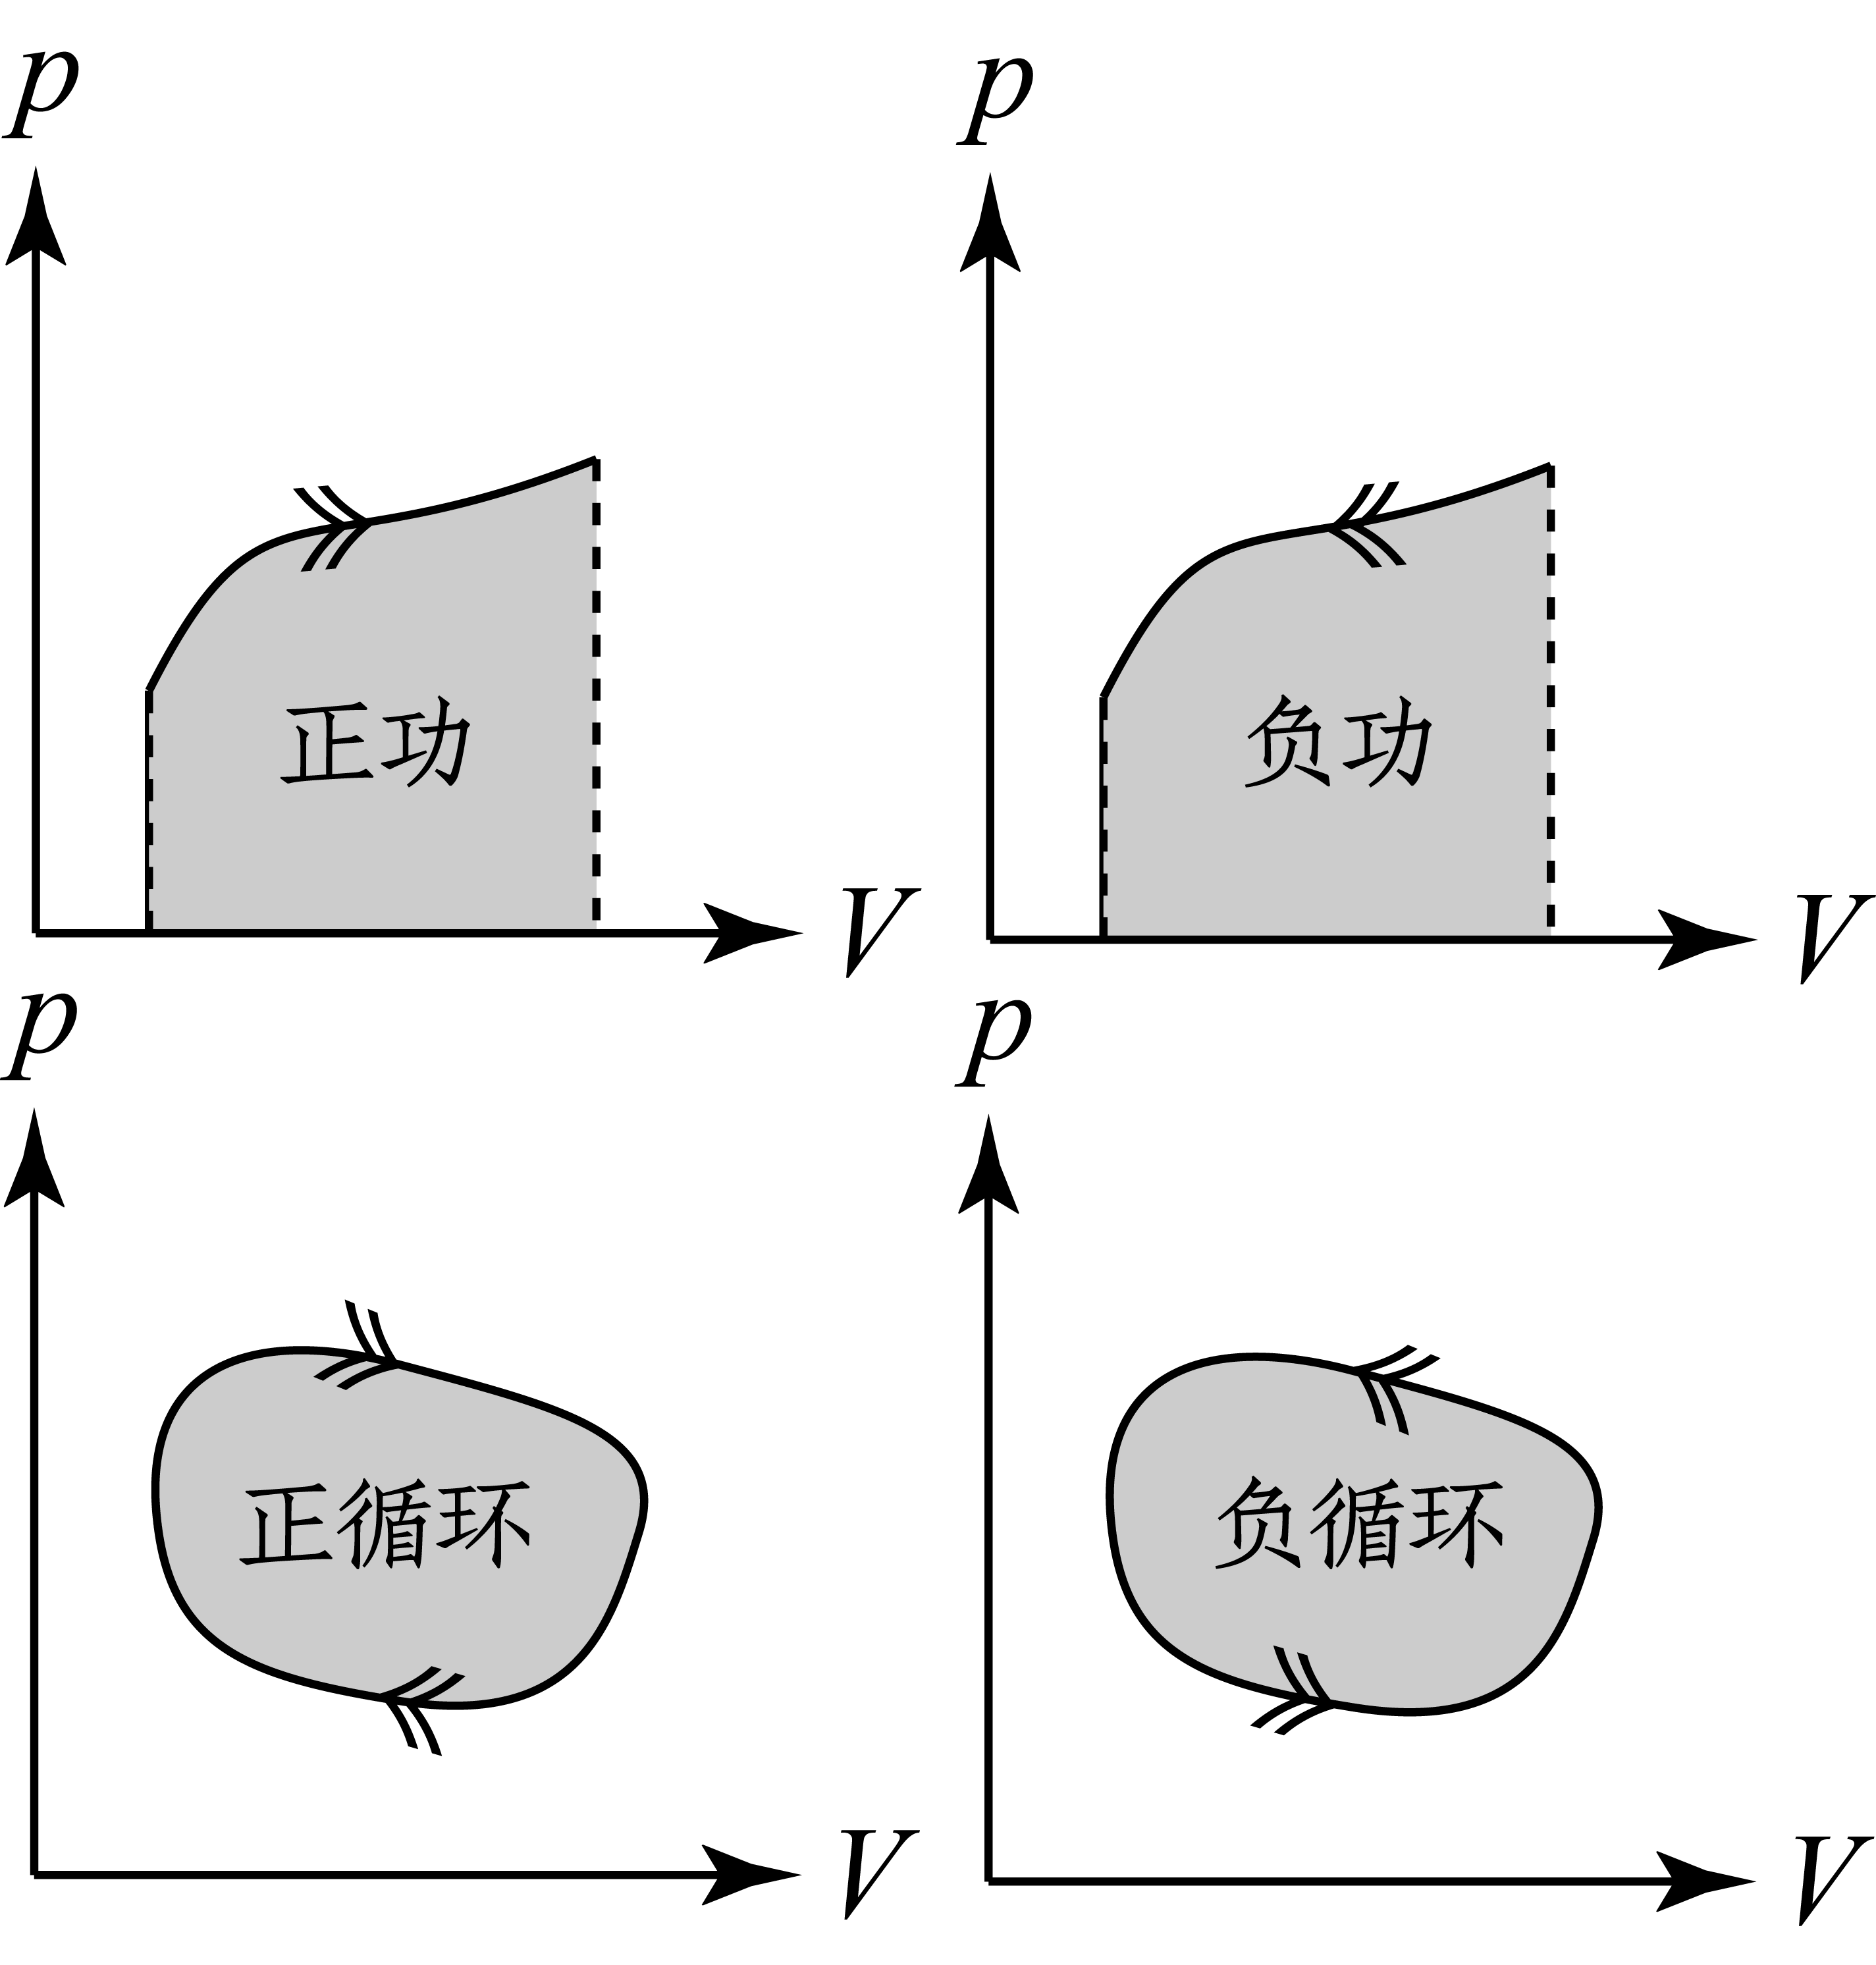
\includegraphics[width=7cm]{image/5-1-1.png}
\caption{准静态过程的做功}
\end{wrapfigure}
对于体积功,\,在准静态过程中可以由$p-V$图下的面积计算.\,在循环过程中则等于过程曲线所包含的面积.\,注意其正负号与过程方向之间的关系.\,但对于非准静态过程.\,做功一定要由外界参数(活塞加速度,\,活塞外气压等)计算而不是用内部气体的过程方程.\,这是因为即使形式地写出内部气体所发生的过程的过程方程.\,由于气体发生膨胀处的压强不等于过程方程中的平均压强,\,对做功的计算是没有意义的.
\subsection{热量}
做功与\emph{传热}(heat transfer)是截然不同的两种向系统注入能量的方式.\,做功依赖于广义坐标这一参数的改变.\,本质上与每一个微观粒子的能量对于广义坐标的依赖有关.\,然而热量则完全不依赖于外在的参数.\,它与系统粒子关于不同能量的状态的占据数\emph{配分}(partition)有关.\,也就是与温度息息相关.\,温度高的物体,\,占据在高能量状态上的粒子较多,\,低能量状态的粒子较少,\,与低温物体发生热接触时,\,单位时间内高能粒子碰撞低能粒子传递能量的可能性更高.\,其统计平均效应就是高温物体向低温物体放热.\,准静态的\emph{等温传热}又是怎样一个过程呢?\,从以上分析可知,\,产生温度梯度是有热传导\footnote{注意,\,广义的热量传递还包括热对流与热辐射.}的必要条件,\,没有了温度差热量的交换也就无从谈起了.\,从这个意义上说,\,实际发生的过程其实都是非准静态过程,\,准静态过程仅仅是一种实际过程的一种近似.\,或是我们虚设的一种模型.\,如在等温传热模型中,\,我们设想只让一个物体的高能粒子与另一个物体的低能粒子发生热接触而实现热传递,\,这无疑会破坏热力学的统计规律\footnote{或是借助于所谓的麦克斯韦妖,\,引入信息熵.},\,但有助于我们理解这个过程的发生机理.

\npg{-10pt}

\subsection{耗散}
\begin{wrapfigure}[14]{o}[-10pt]{7cm}
\centering
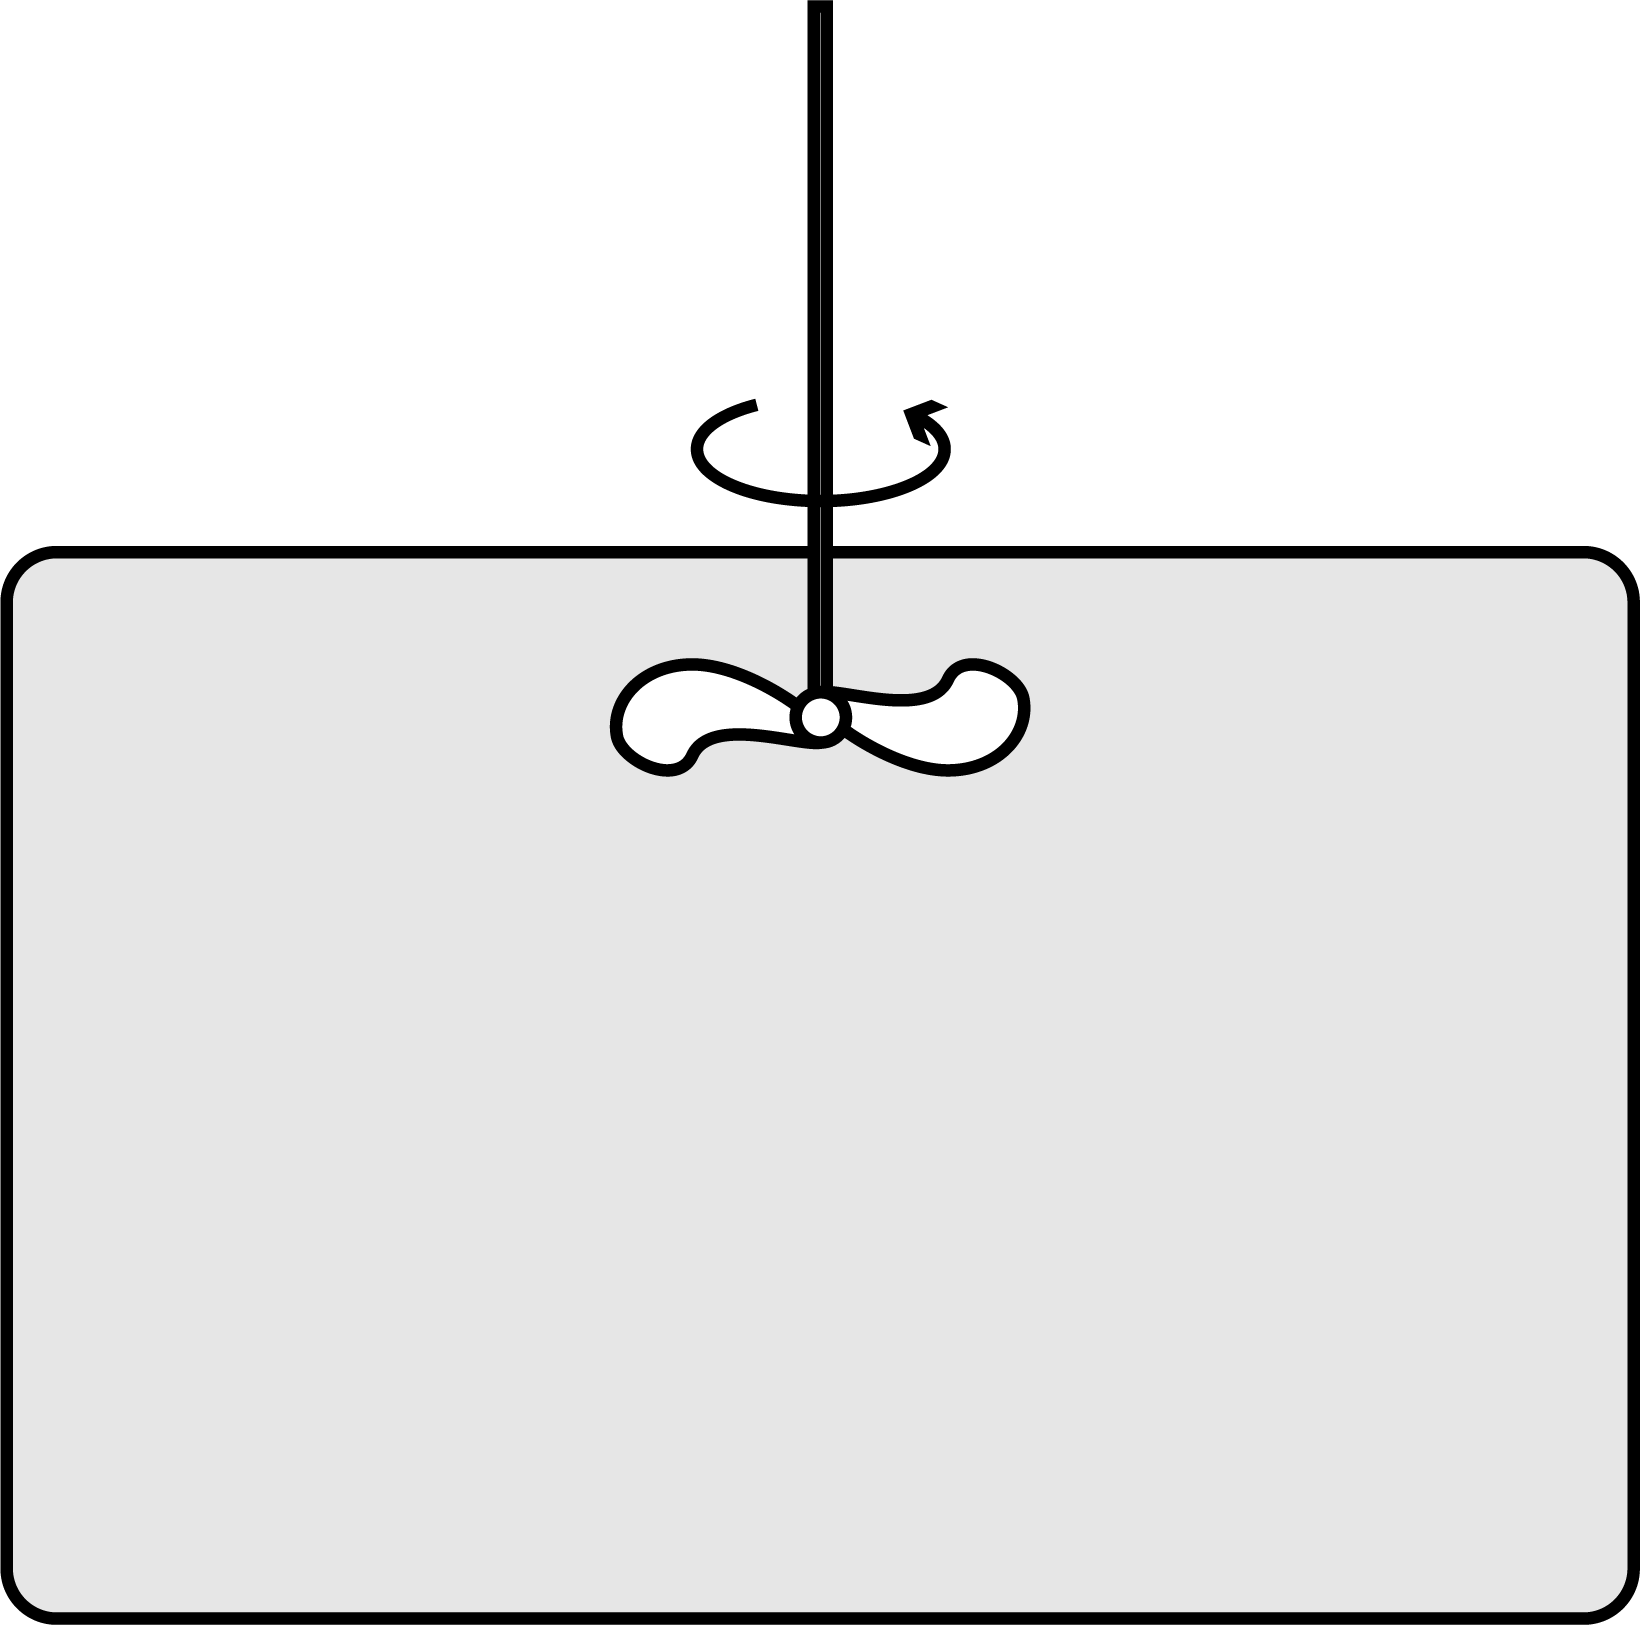
\includegraphics[width=6cm]{image/5-1-2.png}
\caption{搅动空气发热}\label{fig:1-2}
\end{wrapfigure}
还有一类向系统输送能量的方式,\,表面上看是功,\,效果上却是热.\,这被我们称为\emph{耗散}(dissipation).\,俗称\emph{功变热}.\,例如常见的摩擦生热过程,\,非弹性碰撞的过程,\,激光泵浦的过程.\,都是典型的功变热的例子.\,我们看一个十分浅显的例子.\,涡轮叶片搅动气缸中的空气使其温度升高.\,在这个过程中,\,涡轮无疑对气体做功,\,但这个做功并不与系统广义坐标的变化相关.\,它的特点是仅仅作用在系统的一个子系统上.\,再由系统倾向于热平衡的趋势把得来的能量平分到系统各个自由度上.\,从而造成了与吸热完全类似的结果:\,广义坐标没有变化,\,但系统从外界获得了能量.

究其原因,\,本质上是因为系统具有了所谓的\emph{耗散结构}(dissipative structure).\,它不把系统看成一个平衡的整体,\,而是有着复杂内部非线性相互作用的对象.\,故输入的功不一定改变体系的广义坐标,\,但像加热一个系统一般,\,增加了系统的内能.

耗散结构的特点之一是外力驱动系统远离平衡态.\,在非弹性的碰撞过程中固体内部的低频弹性波的成分被突然增强,\,而激光发射的过程中大量粒子被输运到亚稳态而实现布居反转,\,这些都破坏了原来热平衡下的布局.\,需要结合动力学与统计方法来讨论这些现象.

特点之二是开放条件下的自组织现象.\,以普利高津({\it Progogine})为首的研究者把生命现象,\,连同研究过程中的很多奇特现象看成是一种耗散结构的结果.\,这些过程伴随着系统与外界连续不断的能量,\,粒子与信息的交换,\,使得微小的涨落可以在具有正反馈的功能结构中被放大,\,使得体系的对称性被破坏,\,形成有组织的自发序.
\begin{figure}[H]
\centering
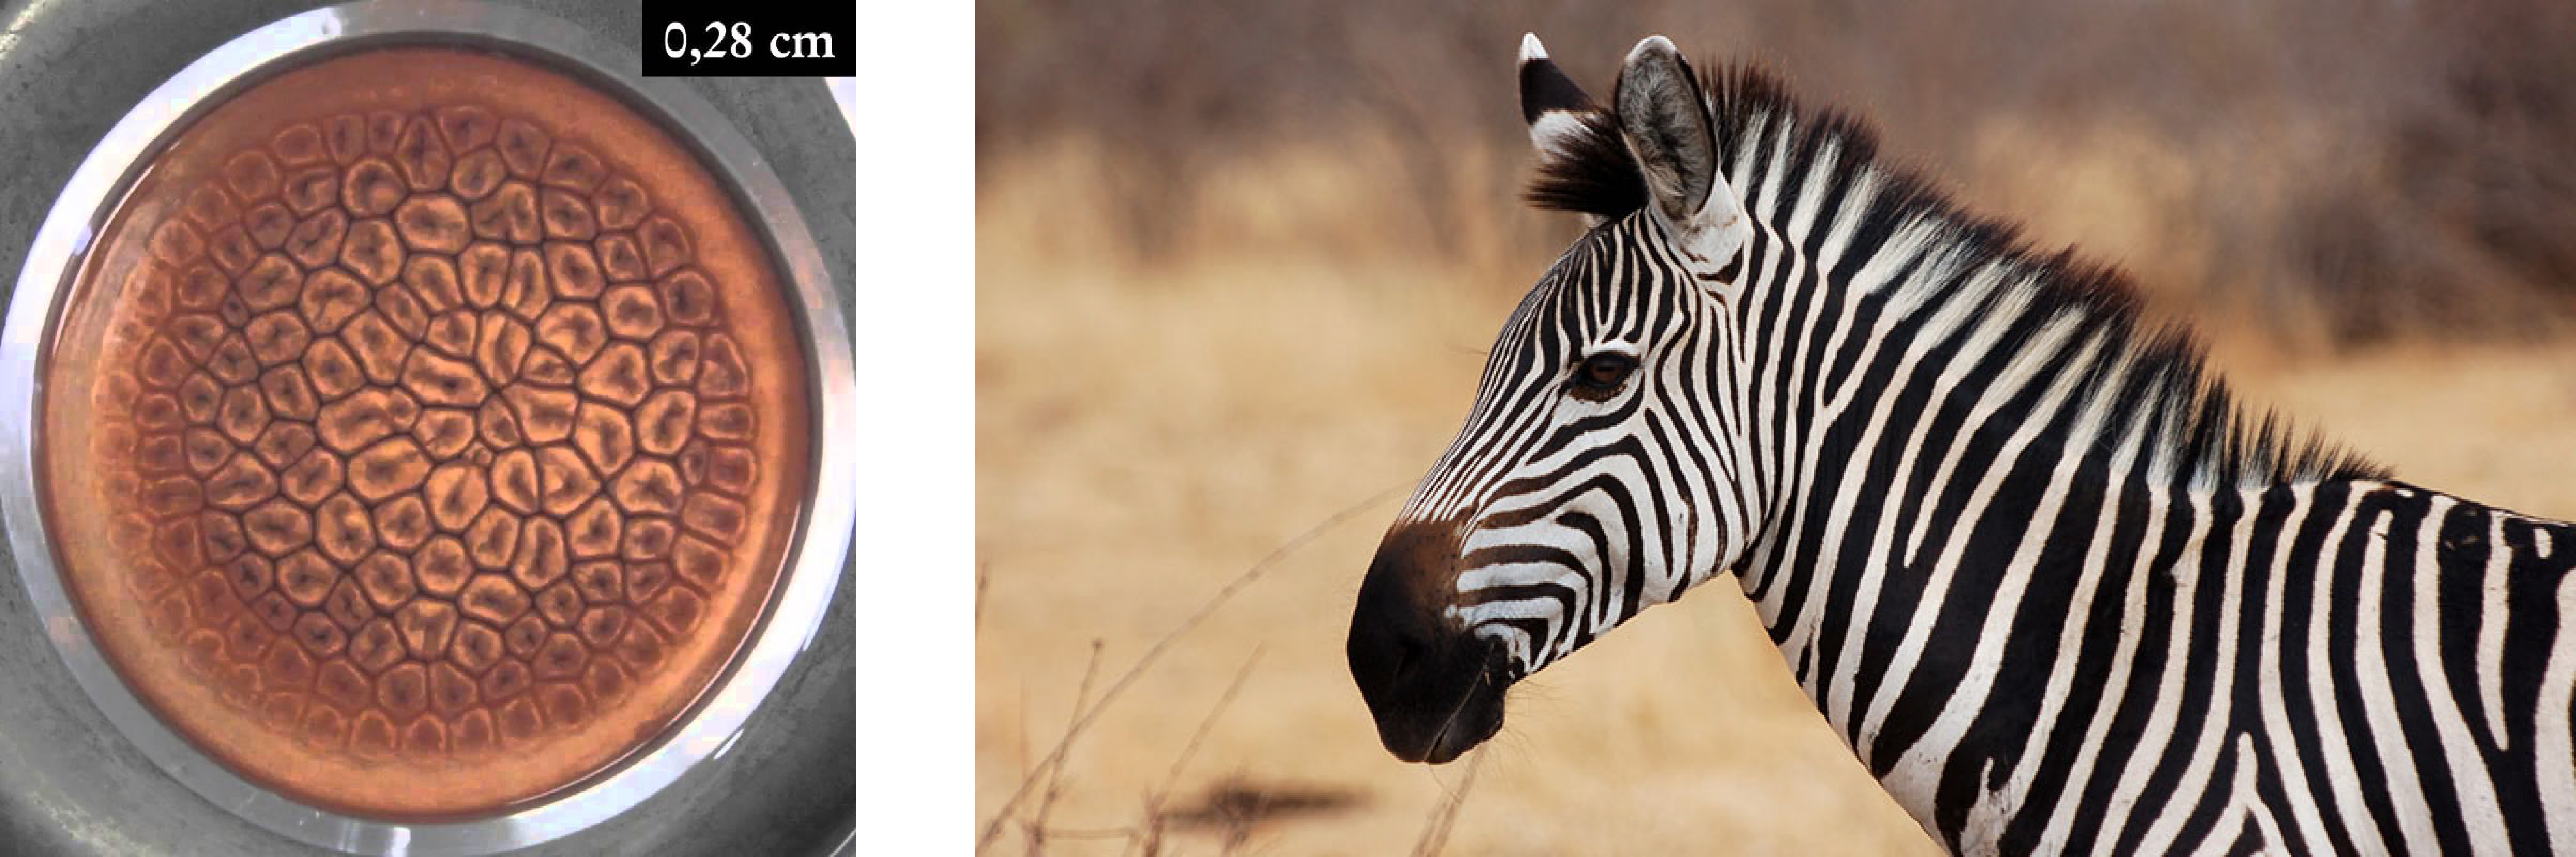
\includegraphics[width=14cm]{image/5-1-3.png}
\caption{自组织现象:\,B\'enard 对流与斑马身上的条纹}
\end{figure}


\npg{-10pt}

\section{理想气体}

\subsection{理想气体的定义}

满足以下三个条件的气体为理想气体:
\begin{enumerate}
	\item 分子间作用力可以忽略;
	\item 分子体积可以忽略;
	\item 分子按自由度平分能量.
\end{enumerate}

我们讨论一下这三个条件.\,首先第一个条件的意思,\,旨在把理想气体间的作用力当成\emph{短程力}(short-range force)处理.\,仅仅当两个分子间距离进入力程范围才可以当做可以发生相互作用(碰撞或散射).\,在这个意义下,\,分子体积实际上也可以处理为半径为力程大小的钢球模型.\,我们忽略这一个体积,\,也就是说所有分子可以自由活动的体积就等于容器体积$V$.\,且分子间相互作用力为零.

然而这两点合在一起将导致一个严重的问题:\,那便是热平衡不可以达到.\,若每个分子不可以通过相互作用或刚性的碰撞与别的分子交换能量与动量.\,那从根本上就不可以达到热平衡,\,统计方法也就无济于事.\,故分子体积足够小,\,小到可以忽略其对热力学性质的影响,\,但又足够大,\,大到在我们关心的时间空间尺度内体系能很快地达到热平衡.\,这才是对这两点的正确理解方式.

我们设分子的速率分布函数为$f(v)$,\,意思是每取$N$个分子,\,速率介于$v$到$v+\ud v$的分子数平均为:
\[\ud N=Nf(v)\ud v\]

从而分子的平均速率与方均速率为:
\[\overline{v}=\int_0^\infty vf(v)\ud v \quad ; \quad \overline{v^2}=\int_0^\infty v^2 f(v)\ud v\]

分子质量为$m$,\,直径为$D$,\,数密度为$n$.\,从中我们得出分子间平均距离$d$:
\[d\sim\frac{1}{\sqrt[3]{n}}\]

\begin{wrapfigure}[15]{o}[-10pt]{7cm}
\centering
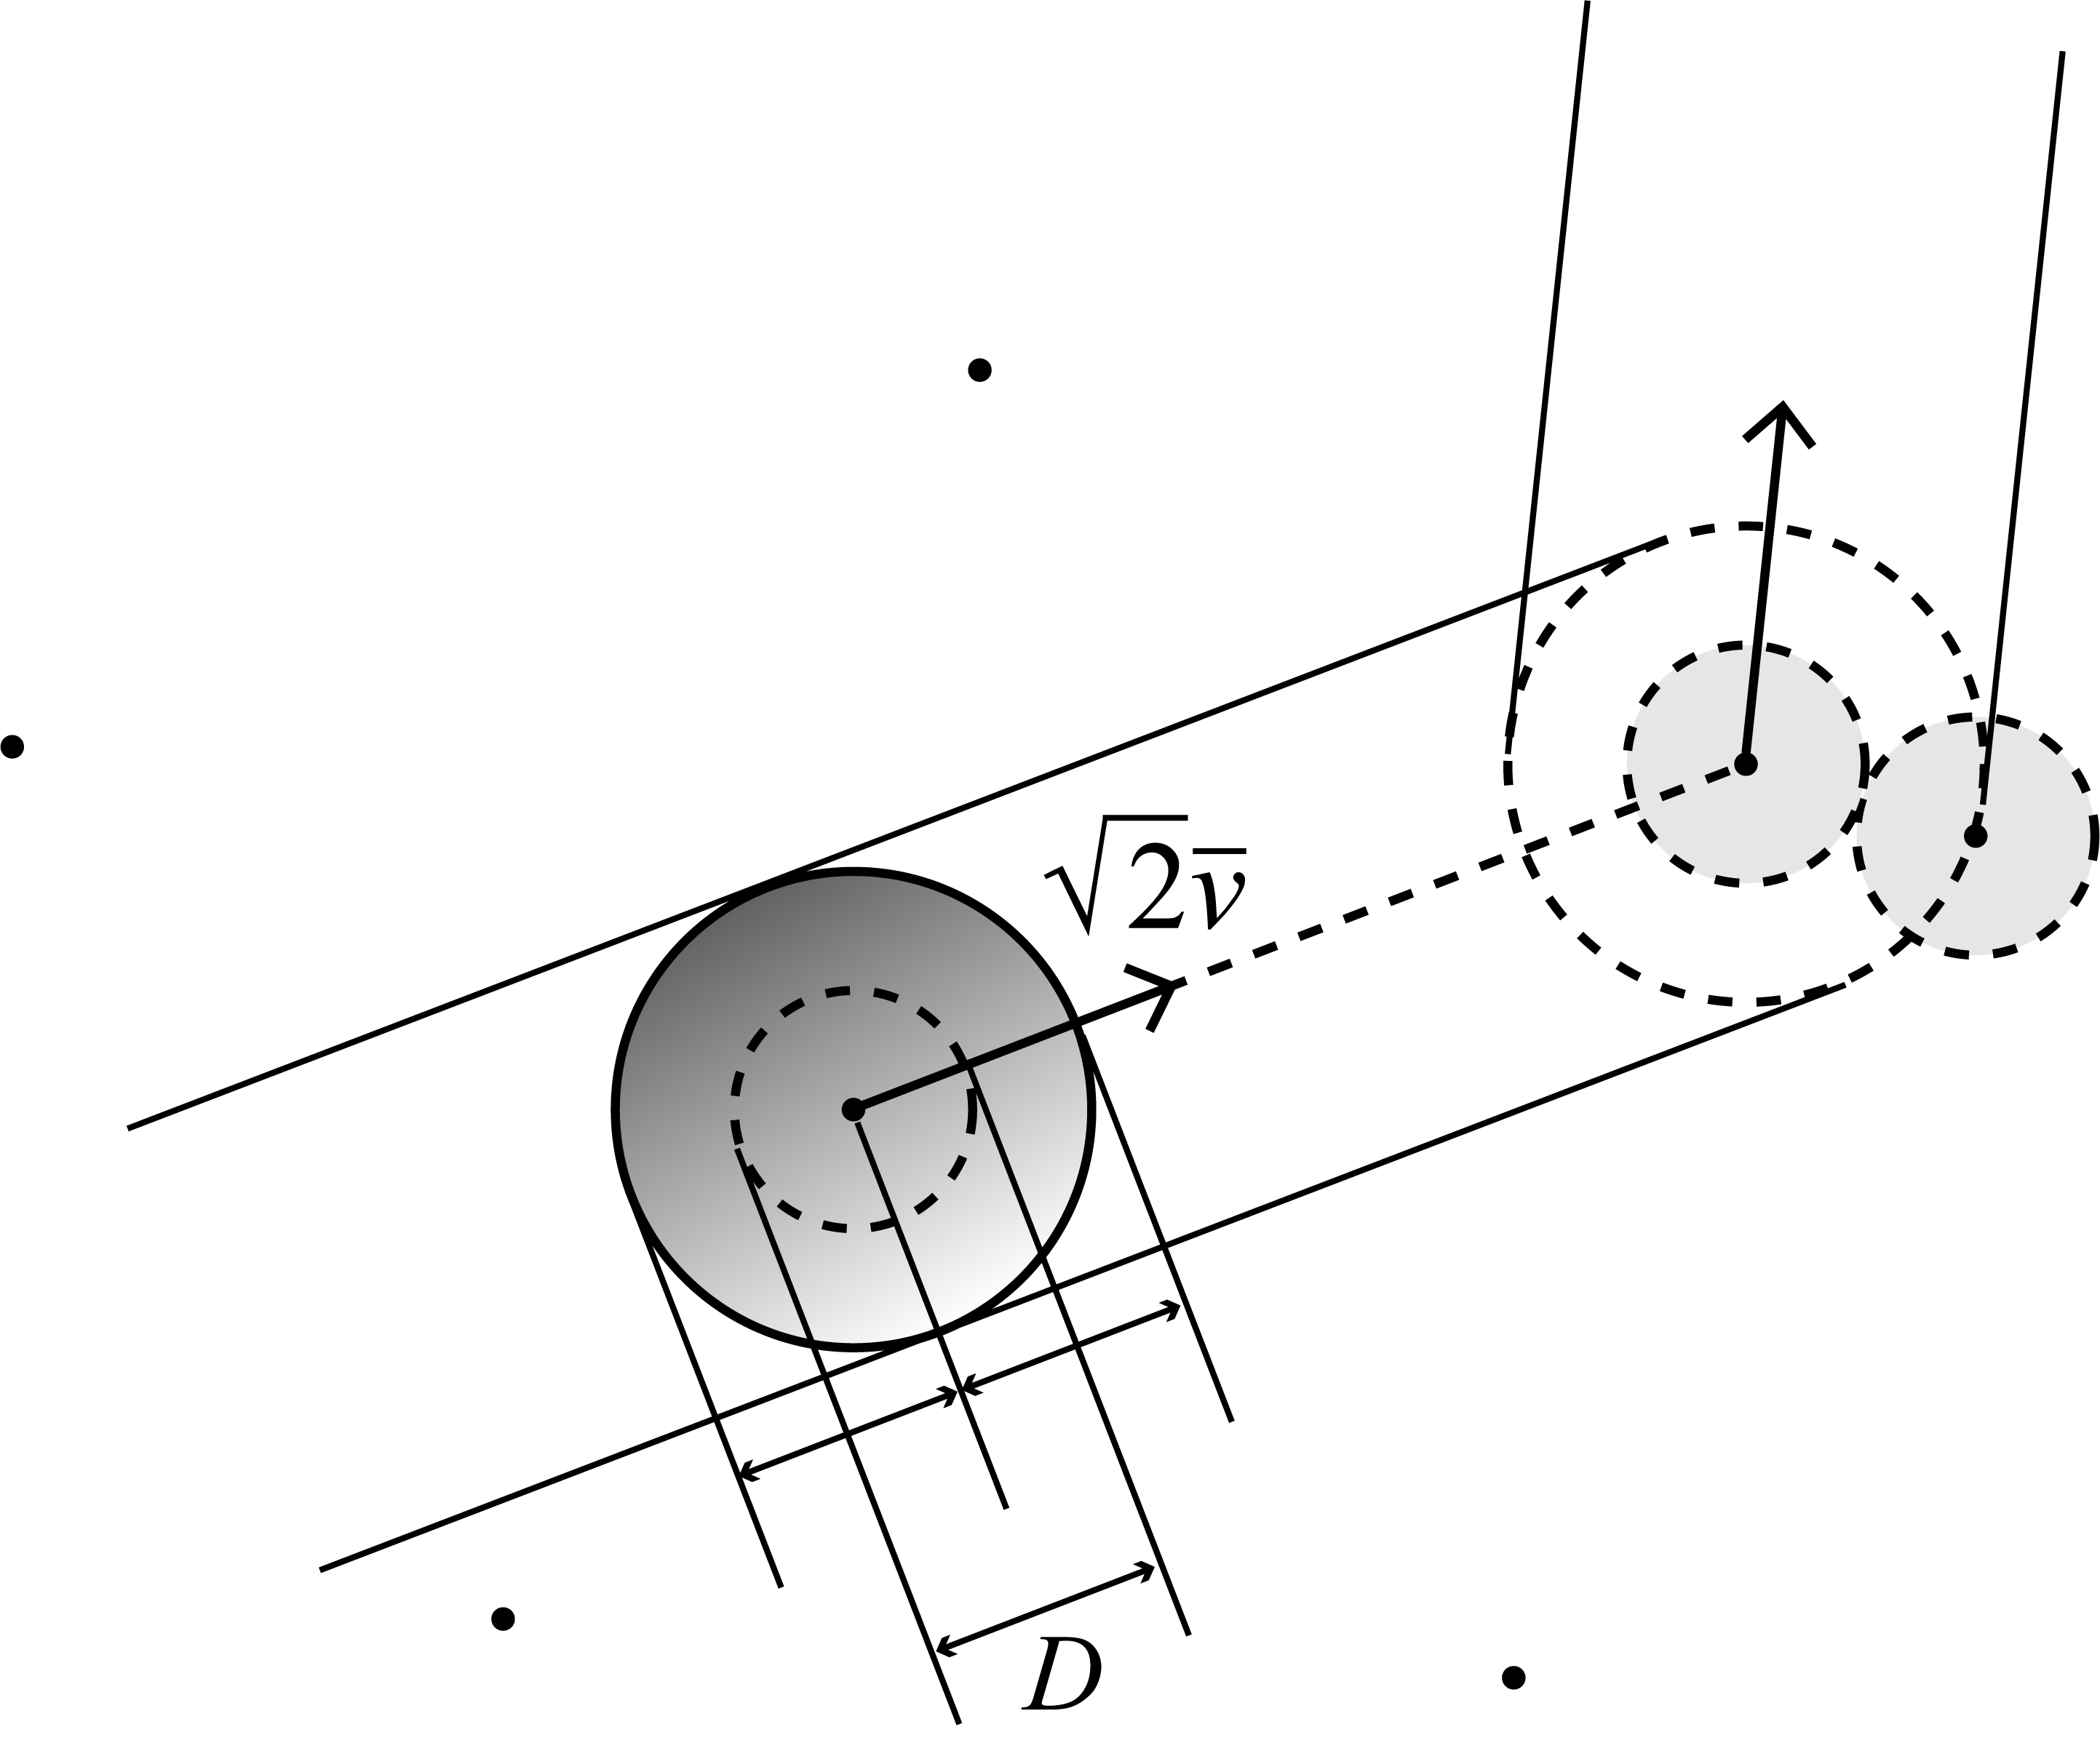
\includegraphics[width=6cm]{image/5-1-4.png}
\caption{曲折柱体计算}
\end{wrapfigure}
可以想见,\,分子间平均距离$d\sim 10{\rm nm}$(大气压下)越大,\,分子直径$D\sim 1{\rm nm}$越小,\,气体越能够近似为理想气体.\,同时其相隔两次碰撞的平均时间间隔$\tau$与空间间隔$\lambda$也会越大.\,如何计算这两个量呢?\,由于分子的速度符合麦克斯韦分布律(参见第五章),\,故两分子间的平均相对速率为$\sqrt{2}\overline{v}$.\,将待研究的粒子处理为钢球,\,速率恒定为$\sqrt{2}\overline{v}$,\,其半径为原分子直径$D$.而其他分子处理为静止的质点,\,半径为零.\,这样钢球碰到质点,\,即相当于原来的两个分子发生碰撞.\,而时间$t$内钢球扫过的体积为:
\[V(t)=\pi D^2\cdot \sqrt{2}\overline{v}t\]

发生碰撞次数$c$:
\[c(t)=nV(t)\]

当$c=1$时,\,对应的时间即为平均自由时间$\tau$,\,又称为\emph{驰豫时间}(relaxation time),\,而这一段时间内粒子走过的距离即为\emph{平均自由程}$\lambda$(mean free path):
\[\tau=\frac{1}{\sqrt{2}\pi nD^2\overline{v}} \quad ; \quad \lambda=\frac{1}{\sqrt{2}\pi nD^2}\]

即有:
\[\lambda\sim\frac{d^3}{D^2}\sim 100d\sim 1{\rm \upmu m}\]

以上数据仅仅在大气压下有效,\,注意平均自由程与分子平均速度无关,\,仅仅是一个几何相关量.\,而它与$n$成反比,\,也就是与$p$成反比,\,如果压强减小到约$1{\rm Pa}$(而温度不变),\,则平均自由程$\lambda$增大5个量级,\,也就是分米量级.

现在我们做一个总结:\,我们取了一个分子间相互作用力与分子的大小可以忽略的模型来研究理想气体,\,它对应的条件是:
\[D \ll d \quad ; \quad \lambda\sim\frac{d^3}{D^2} \ll L\]

第一个条件是保证分子体积可以忽略,\,第二个条件是在研究的问题尺度内保证分子有足够的空间来实现动量能量交换以达到热平衡.

现在让我们专心研究第三个条件.\,能量按自由度均分是麦克斯韦分布的一个独特结果.\,详情也可以参见第五章.\,现在我们指出,\,由于系统中的各个自由度,\,如$x,\,y,\,z$方向的平动,\,分子的转动,\,振动的能量具有相似的形式\footnote{指谐振子形式,\,详见第五章.},\,而且可以通过相互作用(碰撞)交换能量,\,总能量守恒.\,在这样的条件下,\,统计规律告诉我们每一个分子每一个自由度上都分得相同的平均能量值.\,这个平均能量值\footnote{及其对应的按能量高低的配分.}即代表了体系的温度:
\[\overline{\varepsilon}=\frac{1}{2}kT\]

体系自由度越多,\,分子数越多,\,在一定温度下储能就越多:
\[U=N\cdot\frac{f}{2}kT\]

其中$f$是系统能量自由度数\footnote{注意其与动力学自由度的区别,\,振动的势能也对应能量自由度,\,但其动力学自由度与振动动能重合.}.\,它被视为与温度无关的常量\footnote{然而实验发现这些不是常量,\,而是随着温度升高越来越大,\,存在一些基本不变的平台,\,思考这意味着什么.}.\,对于上式,\,我们再引入\emph{摩尔}(mole)这一化学计量单位来表示巨大的原子数$N$:
\[\frac{N}{N_A}=\nu \quad ; \quad N_A=6.022140857\pow{23}/{\rm mol}\]

同时,\,普适气体常量被定义为:
\[R=N_A k=8.314{\rm J/mol\cdot K}\]

这样气体的内能即为:
\[U=\frac{f}{2}\nu RT\]

\subsection{理想气体物态方程}
我们发现,\,$\ud p_1=f(v)\ud v$表示的含义为任意一个分子的速率落在$v\sim v+\ud v$区间内的概率.\,然而对于这样的分子,\,它速度方向在空间中的取向是任意的,\,各向同性的.\,所以建立极轴后,\,速度与极轴夹角在$\theta\sim\theta+\ud \theta$范围内的概率又为:
\[\ud p_2=\frac{\ud \Omega}{4\pi}=\frac{2\pi\sin\theta\ud\theta}{4\pi}=\frac{\sin\theta\ud\theta}{2}\]

对于这样的分子,\,它在容器中的任何位置都是有可能且等概率的,\,所以出现在体积微元$\ud V$中的概率还有$\ud p_3$,\,联合概率为$\ud p=\ud p_1\ud p_2\ud p_3$.

\begin{wrapfigure}[12]{o}[-10pt]{6cm}
\centering
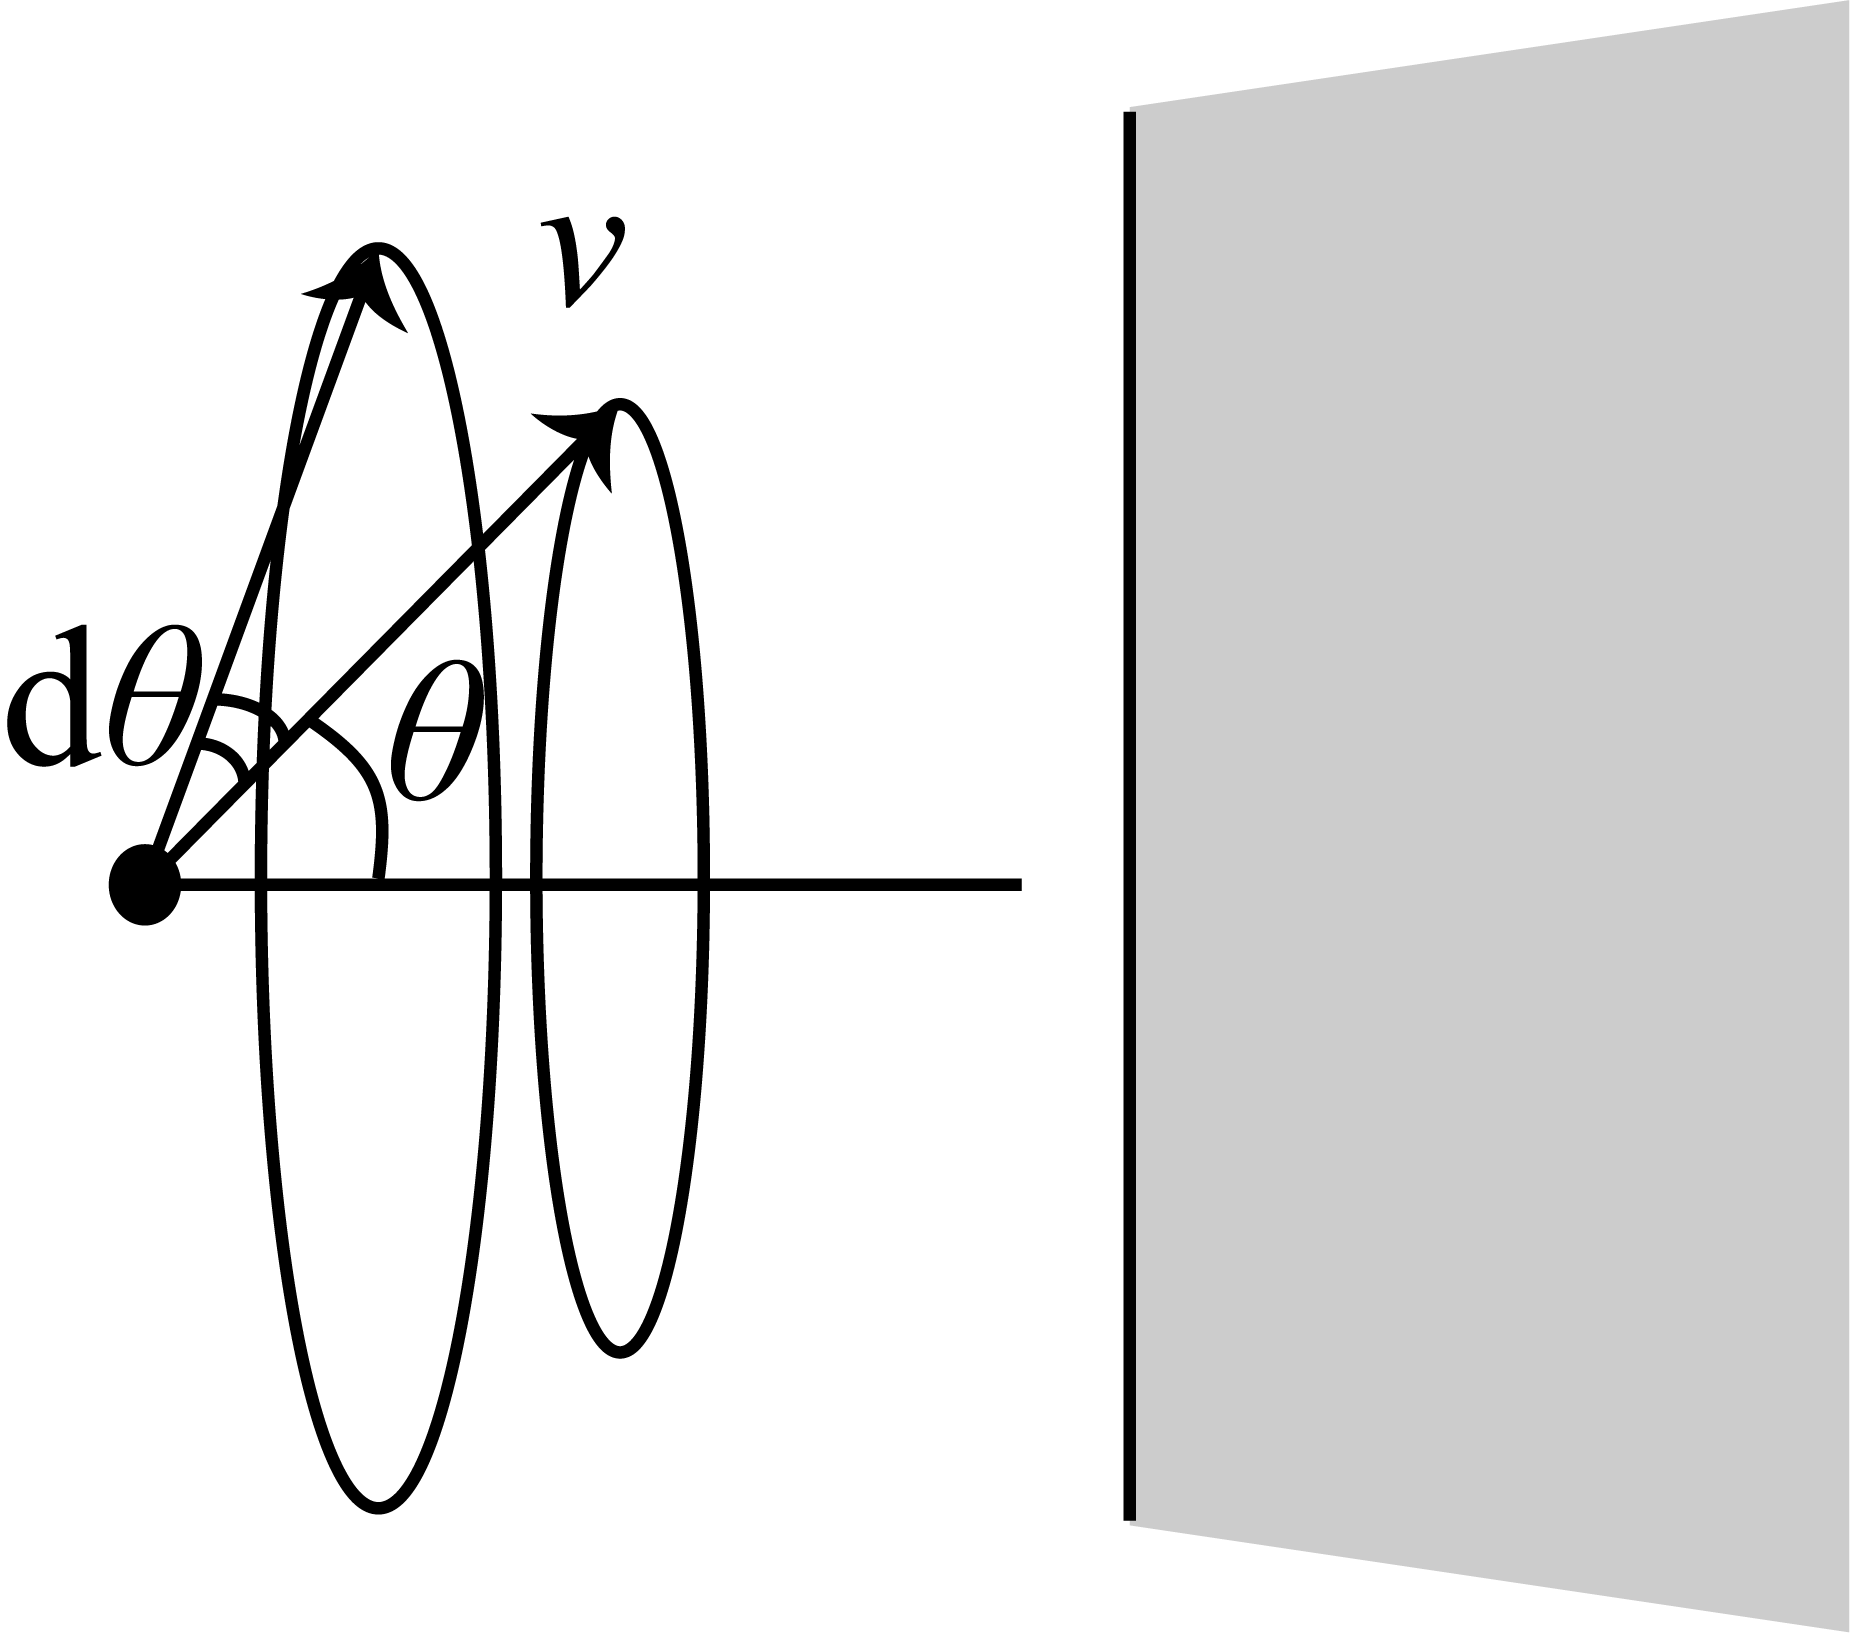
\includegraphics[width=6cm]{image/5-1-5.png}
\caption{粒子速度方向分布}
\end{wrapfigure}
我们接下来考虑气体的压强.\,在这之前我们了解两个概念是十分有帮助的:\,处于平衡态的系统可以看成互相达到平衡的各部分\emph{子系统}(subsystem)直接组成.\,这些部分的所有\emph{强度量}(intensive property)都是完全一致的,\,如理想气体的压强,\,温度,\,粒子数密度,\,摩尔体积,\,摩尔内能等等.\,而子系统的\emph{广延量}(extensive property)大小之和即为总系统的对应量的大小,\,如分子数,\,摩尔数,\,体积,\,内能,\,焓等等.\,我们可以这么理解:\,强度量描述体系的内禀属性,\,而广延量仅仅反应全同子系统的简单堆积.\,如一杯盐水,\,确定了我们关心的强度量\ca 温度和浓度之后,\,我们就可以回答``怎样的盐水''这一个问题.\,而接下来只需要再回答``有多少''这一个简单的问题,\,就能算出所有的广延量来.\,基于这一点理解,\,我们可以发现以下两个性质是成立的:\\[1pt]

{\hei 保持所有强度量不变,\,一个广延量变化$\lambda$倍,\,所有广延量随之变化$\lambda$倍.}\\[1pt]

{\hei 两个广延量之比为强度量,\,典型的如质量$M$比体积$V$为密度$\rho$,\,体积$V$比摩尔数$\nu$为摩尔体积$v$等.}\\[1pt]

理想气体作为极其简单的系统,\,它的独立强度量仅仅只有两个.\,一是系统的温度$T$.\,它决定了分子的平均热运动剧烈程度,\,也就是平均能量大小.\,另一个就是分子数密度$n$,\,它反映单位体积里有多少个全同单元,\,是一种``浓度''.\,其他所有强度量都是这两个量的导出.\,比如压强$p$,\,用分子动理论的方法:
\begin{eqnarray*}
p 	&=&	\int_0^{\infty}\int_0^{\frac{\pi}{2}}n\ud S v\cos\theta\ud t \cdot f(v)\ud v \cdot\frac{\sin\theta\ud\theta}{2}\cdot 2mv\cos\theta/\ud S\ud t 	\\
	&=&	nm\cdot\int_0^{\infty}v^2 f(v)\ud v \cdot \int_0^{\frac{\pi}{2}}\sin\theta\cos^2\theta\ud\theta	\\
	&=& \frac{1}{3}nm\overline{v^2}		\\
	&=& \frac{2}{3}n\overline{\varepsilon_k}	\\
	&=& nkT
\end{eqnarray*}

可见对容器壁的压强正比于温度和分子数密度,\,这一点的物理图像还是很直观的.\,这个压强被我们称之为\emph{外压强}(outer pressure).\,它是由于分子碰撞容器壁引起.\,还有所谓的\emph{内压强}(inner pressure)的概念,\,它由于分子间的碰撞引起.\,理想气体的内压强与外压强相等\footnote{然而范德瓦尔斯气体则不然,\,详见第四章.}.\,但如果气体足够稀薄,\,以至于容器尺度与分子平均自由程可以比拟.\,此时内压强的概念也失去了意义,\,这意味着气体完全不可以用动力学方法处理,\,压强的梯度不会导致气体团的加速度,\,而是以下面所介绍的泻流的方式进行.

上文我们推出来的关系式被称作(强度量之间的)\emph{物态方程}(equation of state),\,它有很多变式,\,如:
\[pV=NkT \quad ; \quad pV=\nu RT \quad ; \quad pv=RT \quad ; \quad p=\frac{\rho RT}{\mu}\]

上面最后一式中$\mu$表示摩尔质量,\,稍作变形还可以得到密度公式:
\[\rho=\frac{\mu p}{RT}\]

用分子动理论方法还可以得到另一个十分重要的量\ca \emph{泻流数}(effusion number).\,如果在容器壁上开一个小孔.\,则速率在在$v$到$v+\ud v$区间内的分子,\,单位面积单位时间通过小孔的分子数为:
\begin{eqnarray*}
\ud \Gamma 		&=& 	\int_0^{\frac{\pi}{2}}n\ud S v\cos\theta\ud t \cdot f(v)\ud v \cdot\frac{\sin\theta\ud\theta}{2}/\ud S\ud t 	\\
				&=&		\frac{n}{2}\cdot \int_0^{\frac{\pi}{2}}\sin\theta\cos\theta\ud\theta	\\
				&=&		\frac{1}{4} nv f(v)\ud v 	\\
				&=&		\frac{1}{4}\ud n v
\end{eqnarray*}
可见速率为$v$的那一部分分子,\,泻流数就是$\ud \Gamma=\frac{1}{4} \ud nv$.\,那么对于所有分子,\,总泻流数为:
\[\Gamma=\frac{1}{4}n\overline{v}\]

泻流的条件是开的孔的大小足够小,\,以至于分子在穿过孔时不会受到别的分子的碰撞.\,也就是其平均自由程$\lambda$显著地大于孔的直径$L$.\,相反地,\,如果$\lambda\ll L$,\,那么就变成了一种压强差驱动气体集团运动的动力学模型,\,我们在下一节阐述.

最后,\,理想气体的内能则可以根据之前关于温度定义的讨论,\,直接写出:
\[U=\nu C_{mV} T\]

其中$C_{mV}$被称为\emph{定容摩尔热容}(molar heat capacity at constant volume).\,其意义之后将了解.\,现在只需知道$\displaystyle C_{mV}=\frac{f}{2}R$.

\subsection{混合理想气体}
考虑几种理想气体的混合,\,我们也需要忽略几种组分分子间的相互作用,\,尤其是应该排除几种分子间发生化学反应的情况\footnote{如混合{$\rm NH_3$}与{$\rm Cl_2$}.}.\,此时,\,几种气体由各自的数密度$n_i$和热平衡下的公共温度$T$描述.\,另一种描述方法是给出总分子数密度$n$与各组分分子所占的比例(强度量)$x_i$:
\[n=\sum n_i \quad ; \quad x_i=\frac{n_i}{n}\]

称为\emph{摩尔分数}(mole fraction),\,注意$x_i$间要满足的归一关系:
\[\sum x_i=1\]

不同组分间分子纵然有碰撞,\,但这对于这一部分分子碰撞容器壁产生的压强大小没有影响.\,也就是说,\,压强等于各组分以$n_i$单独存在时对容器壁产生的分压$p_i$.\,这叫做\emph{道尔顿分压定律}({\it Dalton}'s law of partial pressures):
\[p=\sum p_i \quad ;\quad p_i=n_i kT=x_i p \quad ; \quad p=nkT\]

值得注意,\,每个分子的质量$m_i$或能量自由度数$i_i$并不影响压强的计算.\,压强单方面地决定于分子数密度与温度(分子平均平动动能.\,分子质量改变的是整个体系的摩尔质量$\mu$,\,取一定体积的气体:
\[M=\nu\mu=\sum M_i=\sum \nu_i\mu_i \quad \Rightarrow \quad \mu=\sum x_i \mu_i\]

其中出现的摩尔数$\nu_i$之比即为分子数密度$n_i$之比,\,而摩尔质量$\mu_i$与分子质量的换算关系也很基础,\,请读者一定要熟练使用:
\[\nu_i : \nu_j=\frac{n_i V}{N_A} : \frac{n_j V}{N_A}=n_i : n_j \quad ; \quad \mu_i=N_A m_i\]

能量自由度数影响的是摩尔内能$u$:
\[u=\nu \overline{C_{mV}} T=\sum u_i=\sum \nu_i C_{mVi} T \quad \Rightarrow \quad \overline{C_{mV}}=\sum x_i C_{mVi}=\sum \frac{x_i f_i}{2}R\]

上面我们定义了平均摩尔定容热容$\overline{C_{mV}}$.\,平均的含义一定是按分子数$n_i$(摩尔数$\nu_i$,\,比例$x_i$)平均.

\subsection{理想气体的过程}
\begin{wrapfigure}[15]{o}[-10pt]{6cm}
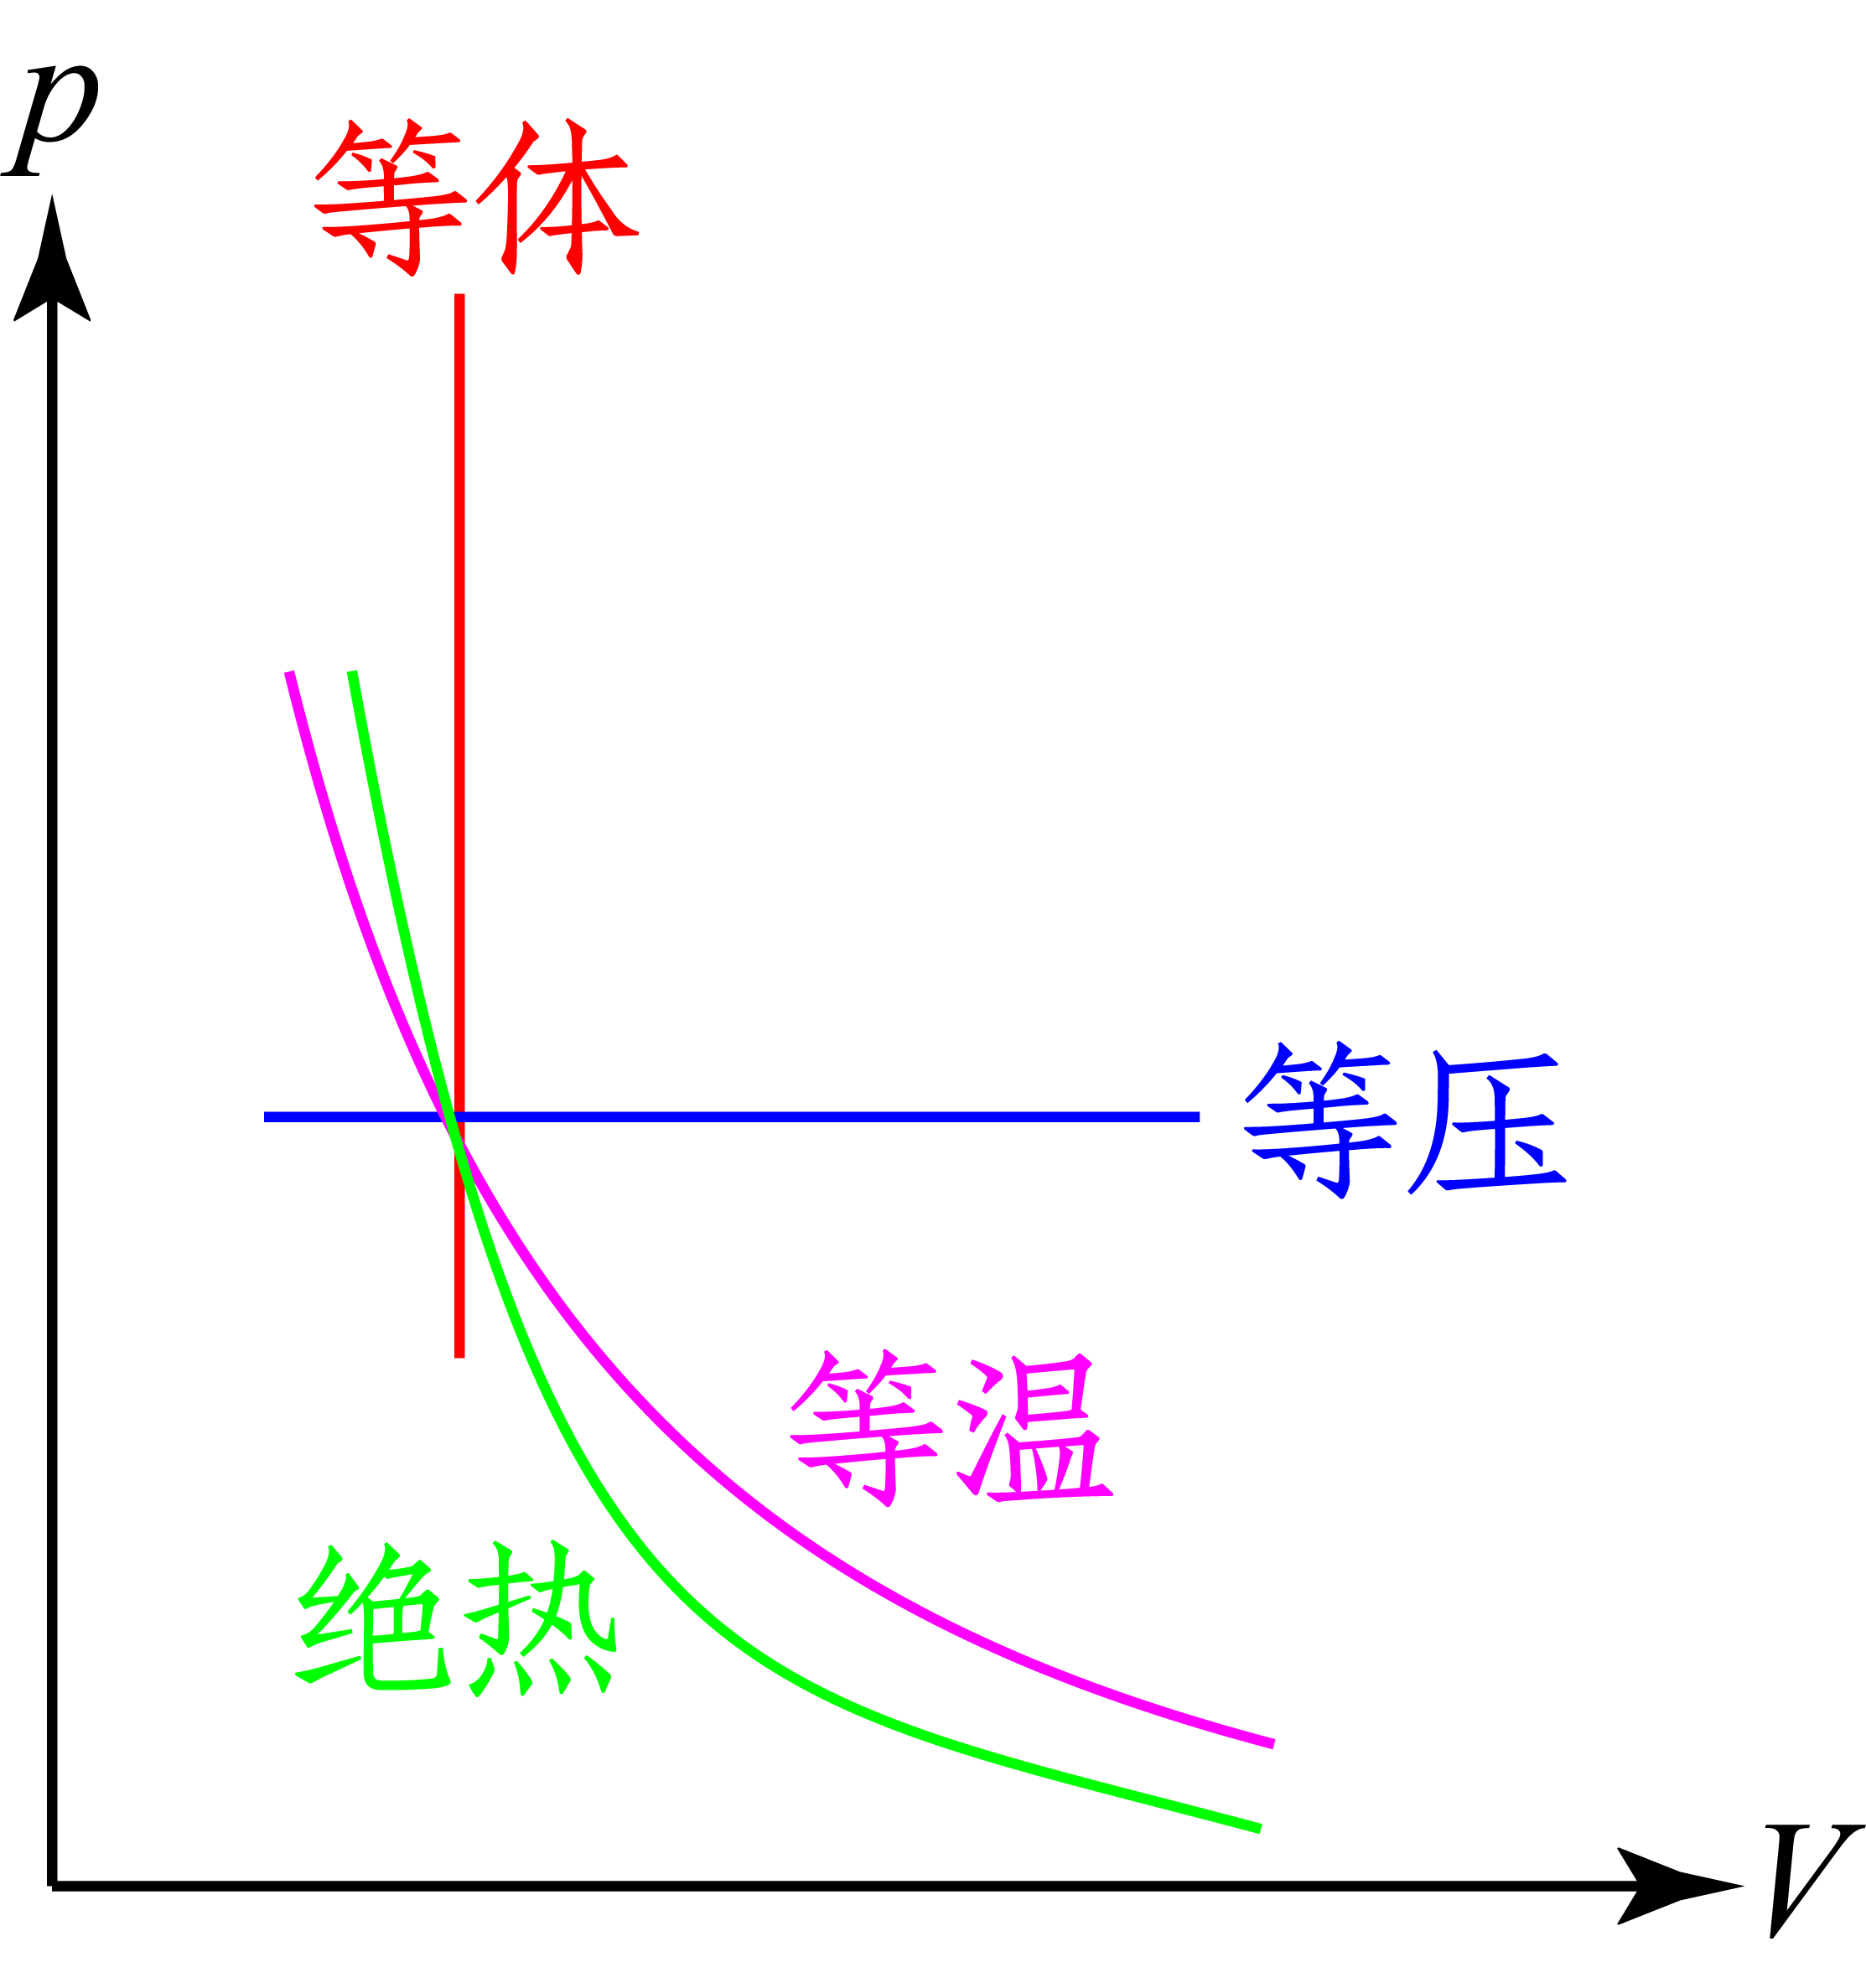
\includegraphics[width=6cm]{image/5-1-6.png}
\caption{四大准静态过程}\label{fig:1-6}
\end{wrapfigure}
所谓\emph{过程}(process)是状态的集合.\,我们考虑的范围内,\,过程的初态和末态都需要是均匀的平衡态.\,中间态如果也可以视为平衡态,\,就叫做\emph{准静态过程}(quasi-static process),\,若中间态蕴含着非平衡,\,则称为\emph{非准静态过程}(non-quasi-static process).\,下面列举常见的过程:
\subsubsection{\hei 等体过程(isochoric process)}
作为等体过程体积功为零$W=0$,\,只能以从外界吸放热$Q$(或是如图\ref{fig:1-2}所示的功变热形式.).\,系统吸热导致温度$T$升高,\,定义系统\emph{热容}(heat capacity)为:
\[C=\frac{\dbar Q}{\ud T}\]

而压强$p$将升高,\,定义\emph{压强系数}(pressure coefficient)为:
\[\beta:=\frac{1}{p}\frac{\ud p}{\ud T}\]

根据理想气体的物态方程与内能公式我们算出\footnote{热力学的角标表示这个量不变,\,而这里热容的表达式下一章学了熵的概念后可以写:\[C=T\frac{\partial S}{\partial T}\]}:
\[C_V=\left(\frac{\dbar Q}{\ud T}\right)_V=\nu C_{mV} \quad ; \quad \beta_V=\frac{1}{p}\left(\frac{\partial p}{\partial T}\right)_V=\frac{1}{T}\]

\subsubsection{\hei 准静态的等压过程(isobaric process)}
若是控制压强$p$而不是体积$V$不变,\,区别在于气体从外界吸收的热量中一部分要用来对外做功:
\[\ud U=\dbar Q-p\ud V\]

热容按同样的方法定义,\,分别称为等体热容和等压热容\footnote{中文太灵活,\,``等体''也有人说成``定体'',\,``等容'',\,``定容''.\,统一术语十分困难.}.\,而\emph{热膨胀系数}(thermal expansion coefficient)定义为:
\[\alpha:=\frac{1}{V}\frac{\ud V}{\ud T}\]

注意这实际上是\emph{体膨胀系数}(volumetric thermal expansion),\,由近似方法可知,\,近似为线膨胀系数$\alpha_L$的三倍.\,对于理想气体等压过程,\,同理可得:
\[C_p=\left(\frac{\dbar Q}{\ud T}\right)_p=\nu (C_{mV}+R)=\nu C_{mp} \quad ; \quad \alpha=\frac{1}{V}\left(\frac{\partial V}{\partial T}\right)_p=\frac{1}{T}\]

\subsubsection{\hei 准静态的等温过程(isothermal process)}
系统与恒温大热库接触,\,吸热膨胀, 压强减小;\,放热收缩,\,压强增大.\,这时$pV$为过程不变量.\,我们定义\emph{压缩系数}(compression coefficient):
\[\kappa:=-\frac{1}{V}\frac{\ud V}{\ud p}\]

注意若是在固体情形,\,以上量被称为\emph{体模量}(bulk modulus).\,对于理想气体,\,等温压缩系数为:
\[\kappa_T=-\frac{1}{V}\left(\frac{\partial V}{\partial p}\right)_T=\frac{1}{p}\]

\subsubsection{\hei 准静态的绝热过程(adiabatic process)}
绝热过程中$\dbar Q=0$,\,对于理想气体:
\[\ud U +p \ud V=0\]
\[\nu C_{mV} \ud T + \frac{\nu R T}{V}\ud V=0\]
\[C_{mV}\frac{\ud T}{T}+R\frac{\ud V}{V}=0\]

惯例上定义\emph{绝热指数}(adiabatic index)$\gamma$为:
\[\gamma:=\frac{C_{mp}}{C_{mV}}=1+\frac{R}{C_{mV}}=\frac{f+2}{f}\]

则可以由$\gamma$和$R$表示两个摩尔热容:
\[C_{mV}=\frac{1}{\gamma -1}R \quad ;\quad C_{mp}=\frac{\gamma}{\gamma -1}R\]

从而我们从绝热过程的热力学第一定律方程积分得:
\[TV^{\gamma-1}={\rm Const.}\]

也可以写为:
\[pV^\gamma={\rm Const.} \quad ; \quad \frac{p^{\gamma-1}}{T^\gamma}={\rm Const.}\]

前一式可以用于在$p-V$图\ref{fig:1-6}上确定过程曲线.\,后一式则注重关心强度量之间的变化关系而不关心广延性质.\,在绝热过程中(用角标$S$表示绝热,\,$S$其实表示熵,\,具体原因见下一章.),\,热膨胀系数,\,压强系数与压缩系数分别为:
\[\alpha_S=\frac{1}{V}\left(\frac{\partial V}{\partial T}\right)_S=-\frac{1}{\gamma -1}\frac{1}{T} \quad ;\quad \beta_S=\frac{1}{p}\left(\frac{\partial p}{\partial T}\right)_S=\frac{\gamma}{\gamma -1}\frac{1}{T}\quad ;\quad \kappa_S=-\frac{1}{V}\left(\frac{\partial V}{\partial p}\right)_S=\frac{1}{\gamma}\frac{1}{p}\]

\subsubsection{\hei 准静态的多方过程(polytropic process)}
多方过程可以由过程方程$pV^n={\rm Const.}$描述,\,多方指数$1<n<\gamma$.\,实际过程若发生缓慢,\,可以近似处理为某种形式的多段多方过程.\,多方过程的热容为:
\[C_{mn}=\left(\frac{1}{\gamma -1}-\frac{1}{n-1}\right)R\]

而其他响应函数(指上面定义的$\alpha$,\,$\beta$与$\kappa$)的形式与绝热过程算出来的类似,\,只需要把$\gamma$改为$n$.\,多方过程在特殊的参数条件下即变成以上过程:
\begin{figure}[H]
\centering
\begin{tabular}{c|c|l}
\hline
绝热指数$n$		&	摩尔热容$C_m$						&	描述			\\ \hline\hline
$n<0$ 			   		&	$\left(\dfrac{1}{\gamma -1}+\dfrac{1}{1-n}\right)R$ 		&	 吸收大量热量,\,压强体积温度同时增加			\\ \hline
$n=0$				  &	$C_{mp}$    																				&   等压过程 		    \\ \hline
$0<n<1$			&   $\left(\dfrac{1}{\gamma -1}+\dfrac{1}{1-n}\right)R$ 				&   相比吸热等温膨胀,\,温度有升高				\\ \hline
$n=1$		&	$\infty$ 																									&  	等温过程 			\\ \hline
$1<n<\gamma$		&	$ -\left(\dfrac{1}{n -1}-\dfrac{1}{\gamma -1}\right)R$ 				& 	膨胀降温时要从外界吸热 			\\ \hline
$n=\gamma$		&	$0$ 																									&	绝热过程 			\\ \hline
$n>\gamma$		&	$\left(\dfrac{1}{\gamma -1}-\dfrac{1}{n-1}\right)R$						& 	压缩气体同时给气体热量的过程	\\ \hline
$n=\infty$		&	$C_{mV}$ 																						&	等温过程			\\ \hline
\end{tabular}
\end{figure}

\subsubsection{\hei 自由膨胀过程}
\begin{wrapfigure}[15]{o}[-10pt]{6cm}
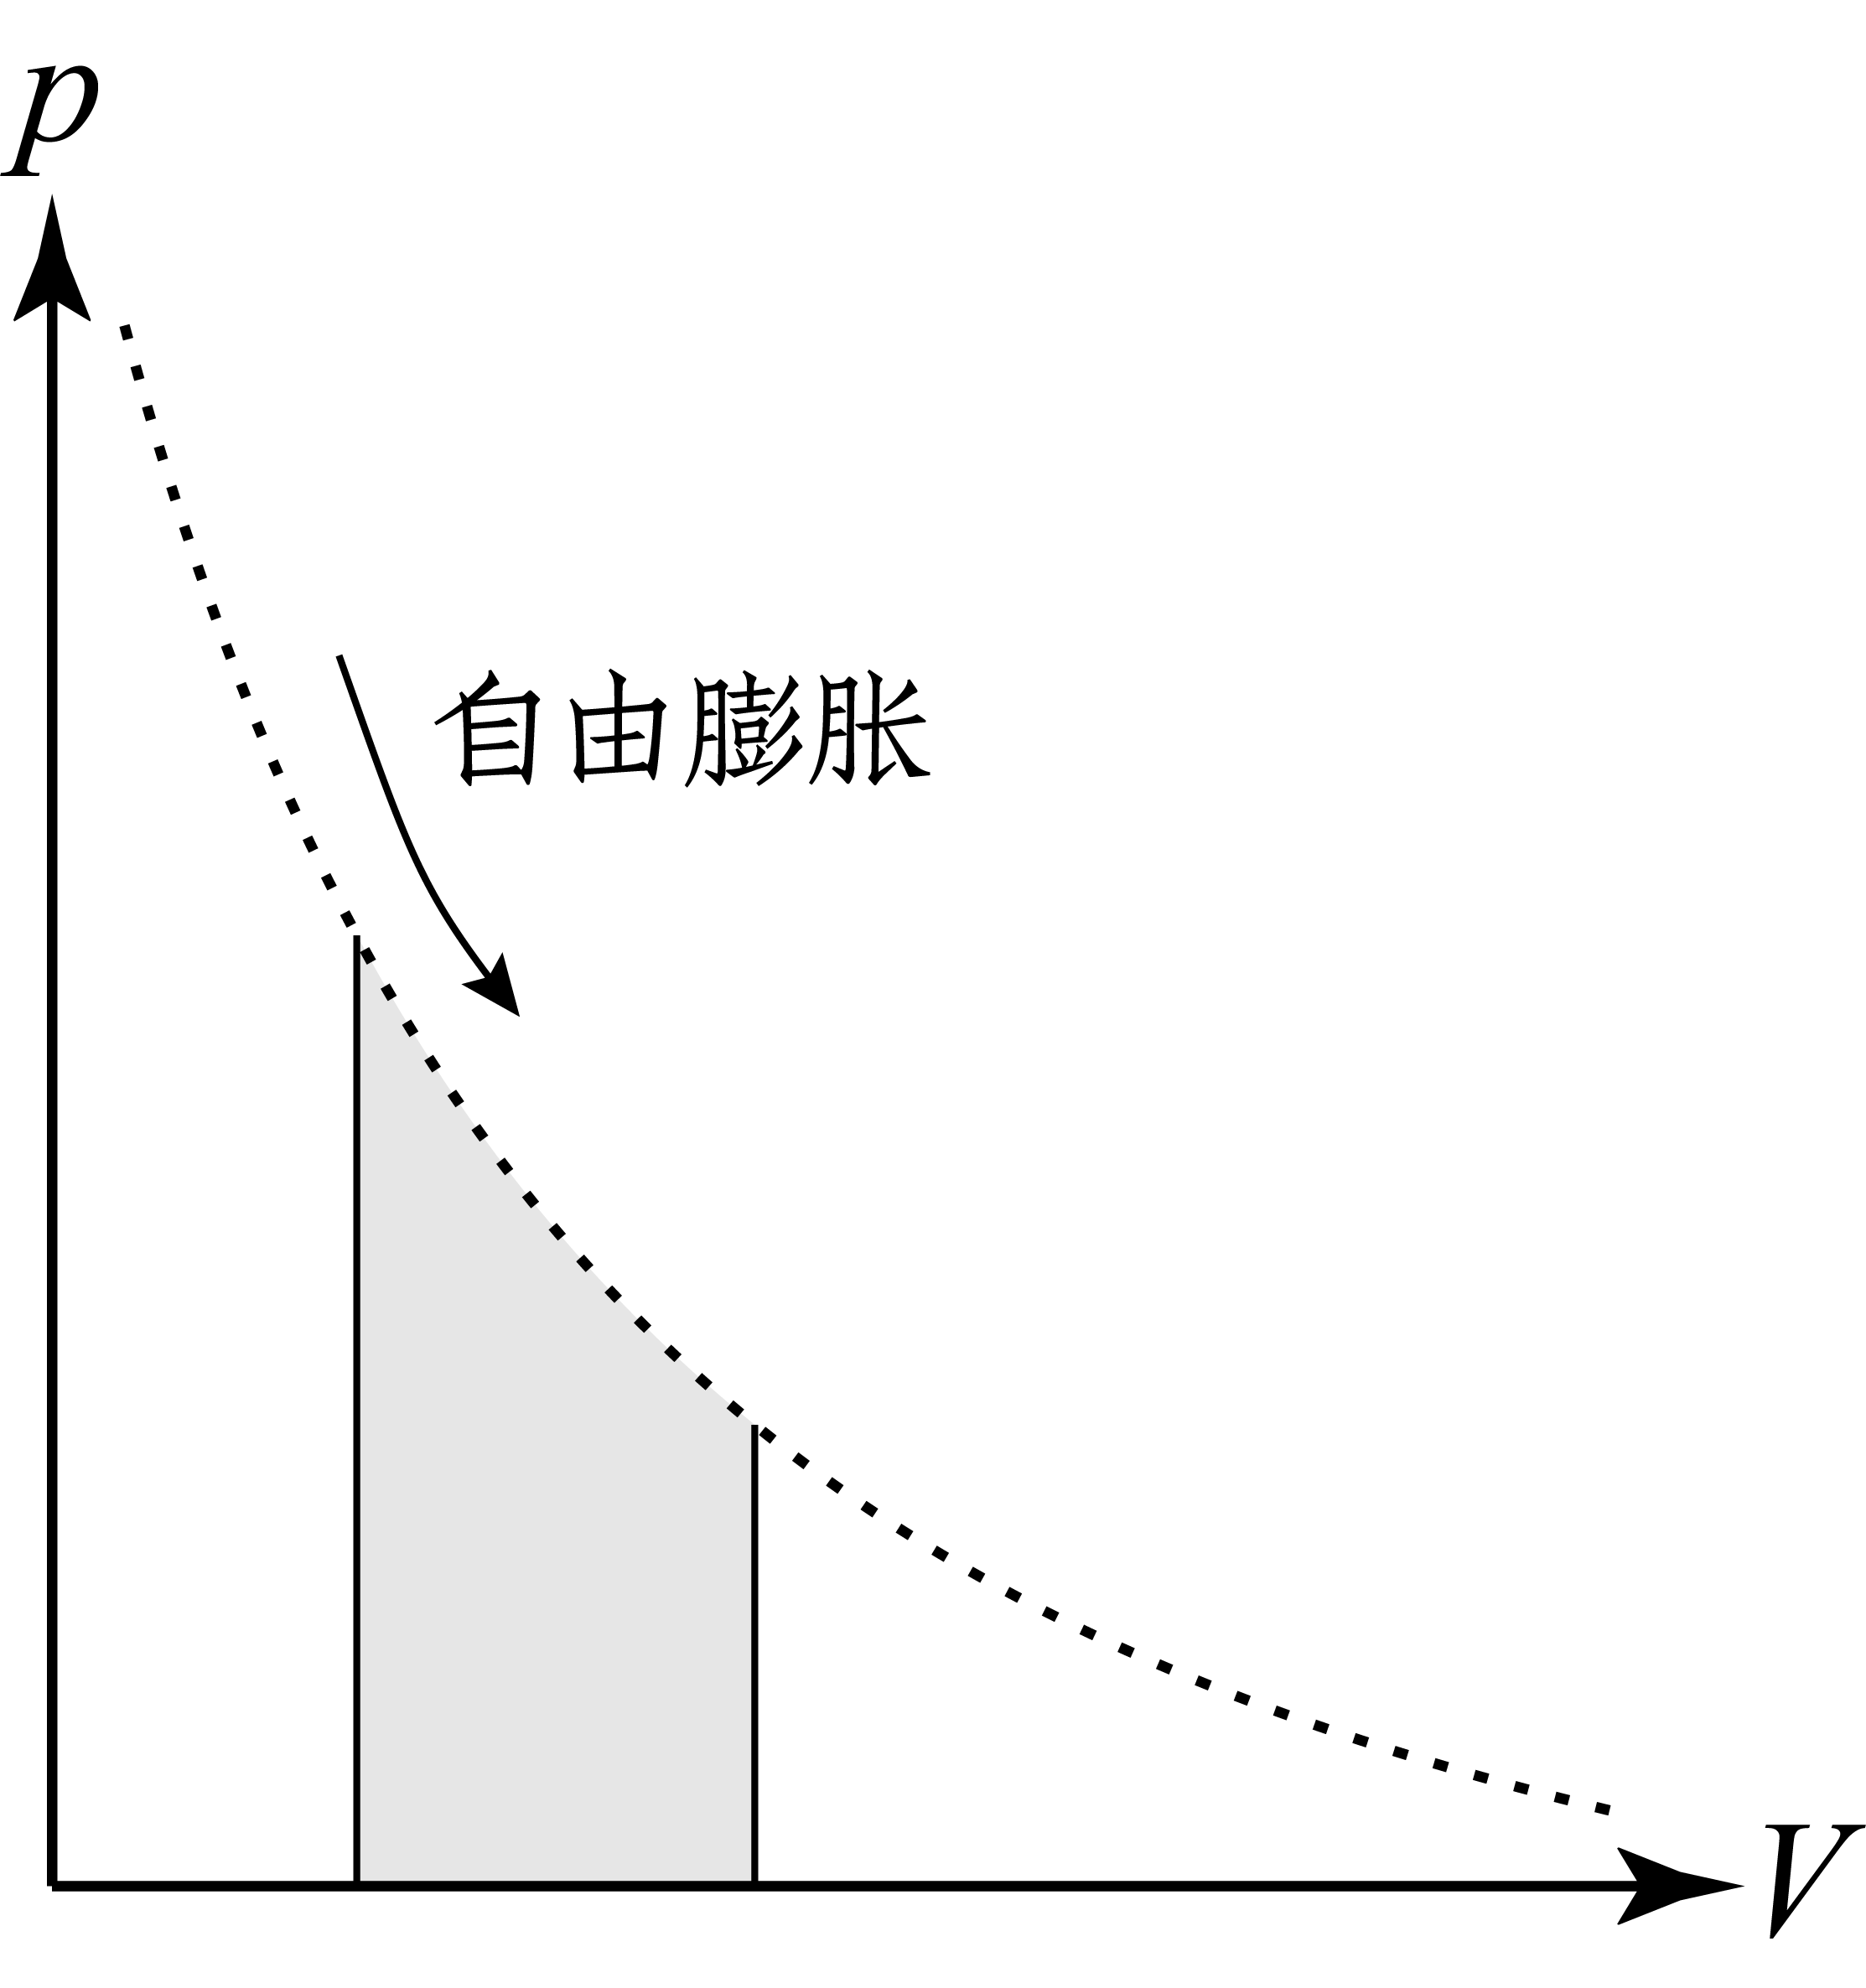
\includegraphics[width=6cm]{image/5-1-7.png}
\caption{$p-V$图上画自由膨胀}
\end{wrapfigure}
理想气体向真空的\emph{自由膨胀过程}(free expansion process)是一类典型的非准静态过程.\,在这样一个过程中,\,由于外压为零,\,外界对气体做功为零.\,而系统绝热,\,从而从外界吸热也为零.\,故由于热力学第一定律,\,内能不变.\,再根据理想气体内能直接依赖于温度的性质,\,我们发现:\,理想气体的自有膨胀是一个非准静态的等温膨胀.

从而在$p-V$图上,\,我们画一根等温线,\,它是否代表向真空的自由膨胀过程?\,我们需要画成虚线,\,线上每一个点都表示平衡态,\,而从一个点到另一个相邻的点中发生的过程则没有达到力学平衡,\,从而不能视为准静态过程.\,这一根虚线能够代表气体在自有膨胀过程中的状态,\,因为即使不均匀,\,整体的内能和可以确定出平均温度,\,整体的体积和平均温度又可以确定出平均压强.\,如果在某个时刻命自有膨胀结束,\,体系达到平衡态后其状态就落在了这根等温线上.\,只不过,\,这根线下面积此时也没有了实际意义,\,因为气体对外做功应该是零.

\vspace{2cm}

\subsubsection{\hei 向固定压强膨胀}
\begin{wrapfigure}[11]{o}[-10pt]{6cm}
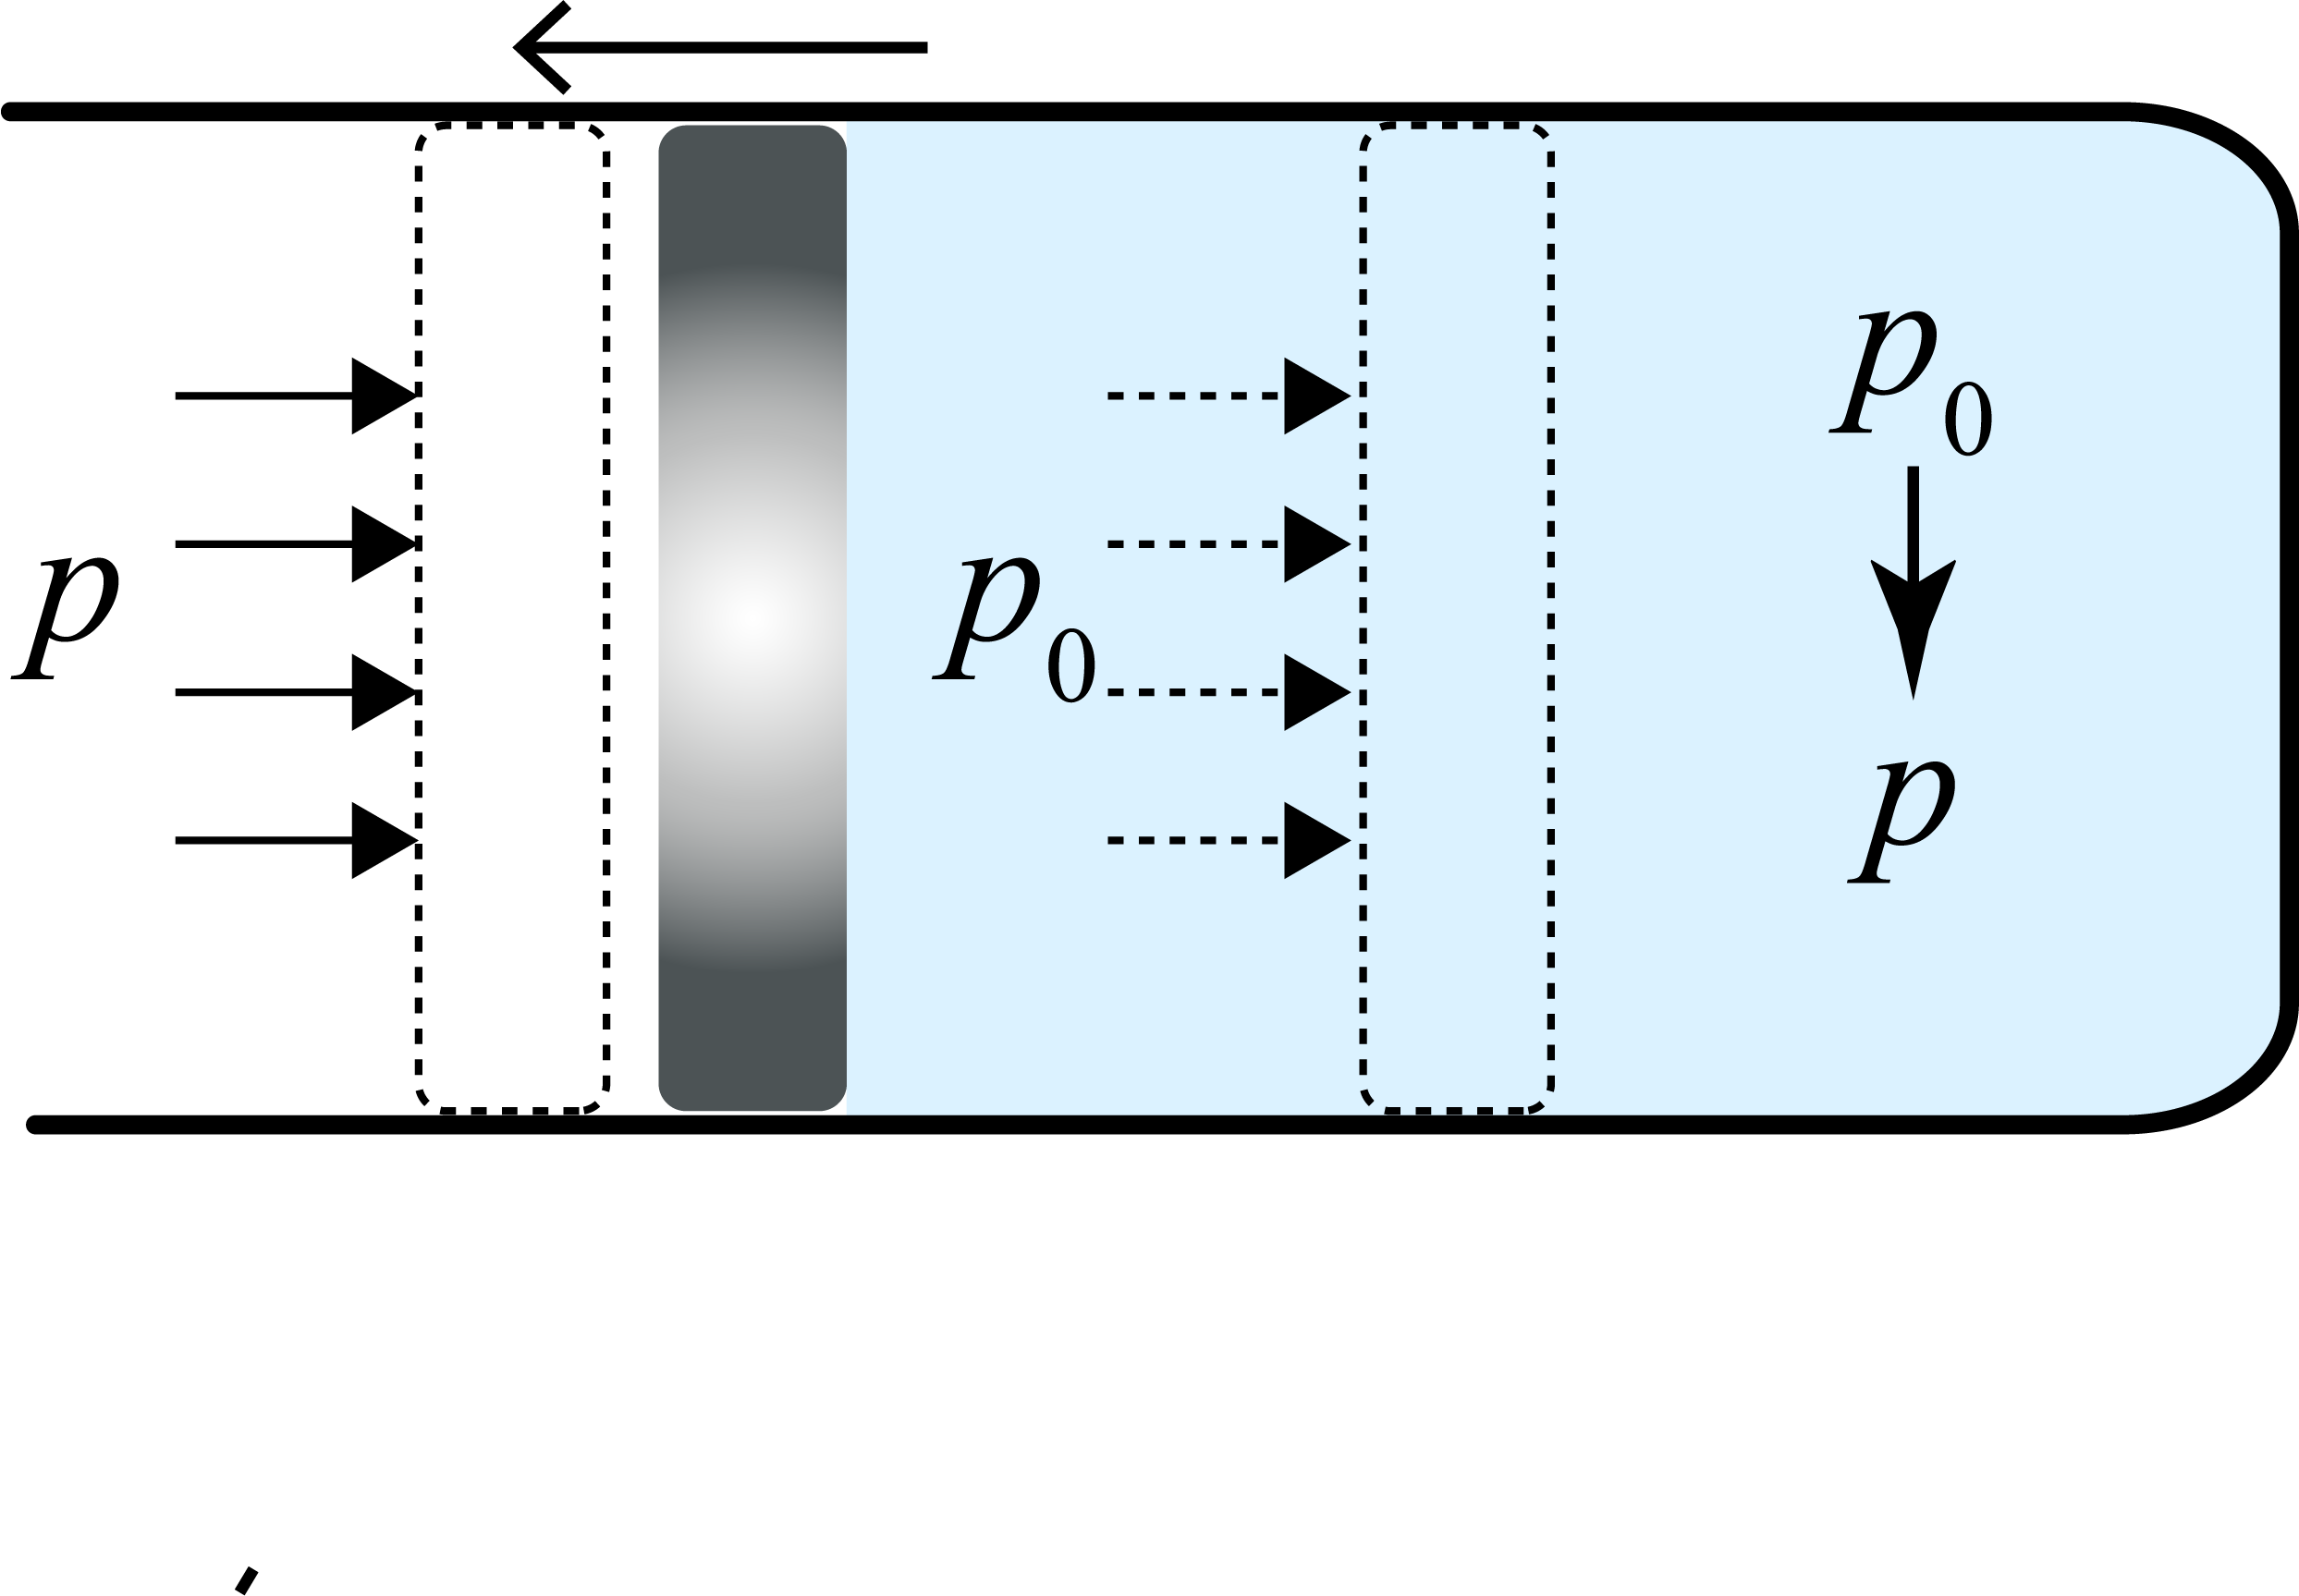
\includegraphics[width=6cm]{image/5-1-8.png}
\caption{向固定压强膨胀}
\end{wrapfigure}
考虑原平衡态压强为$p_0$的气体,\,突然命外压变小为$p$,\,气体将发生某种膨胀,\,如果膨胀稍过度,\,其压强小于外界压强$p$时,\,又会被压缩,\,这样来回振动,\,直到达到新的平衡态.\,如果这个过程系统绝热,\,则系统对外界做功应该写为:
\[W=p(V-V_0)\]

这一个模型可以这样理解:\,它保证了外界压强$p$的严格不变性.\,内部气体由于发生了急剧的体积变化,\,最靠近活塞的部分气体压强由于急剧的膨胀实际上就会等于外界气压$p$.\,这是忽略活塞质量(轻活塞)的情形.\,若是考虑活塞的质量,\,这个结论也还是成立,\,因为内外气体对活塞做功之和转化为活塞动能.\,而前后平衡态活塞实际上动能都是零.\,故内部气体对外做功可以由外界固定压强部分气体的体积功来计算.\,这就是上式.\,那么同样,\,由热力学第一定律和理想气体的性质,\,我们有:
\[\frac{V}{V_0}=1+\frac{p_0-p}{\gamma p} \quad ; \quad \frac{T}{T_0}=\frac{1}{\gamma}+(1-\frac{1}{\gamma})\frac{p}{p_0}\]

如果我们在初态压强$p_0$与末态压强$p$之间搭设很多的压强平台$p_i$,\,使得外压是缓慢地从$p_0$逐级减小到$p$,\,那么用极限的方法容易证明(请读者自己完成),\,过程恰好变为准静态的绝热过程:
\[pV^\gamma=p_0V_0^\gamma \quad ; \quad \frac{p^{\gamma-1}}{T^\gamma}=\frac{p_0^{\gamma-1}}{T_0^\gamma}\]

此时屡次的非平衡态将无限趋于平衡态,\,而非准静态过程也就无限趋于准静态过程了.

\npg{-2cm}

\subsubsection{\hei 节流过程(throttling)}
节流过程亦是对很多复杂系统过程的抽象,\,如冷凝机内部工作物质所发生的循环的定常流动.\,我们从中提取出一个模型,\,如下图,\,气体在内壁光滑的管道内做定常流动,\,通过一多孔塞后压强减小,\,气体膨胀.\,整个过程绝热.\,我们取一个固定的气团(图中红加蓝)作为研究对象.\,经过一定时间$t$后左侧与右侧体积变化分别为$V_1$与$V_2$,\,那么气体的流量被定义为:
\[Q=\frac{m_i}{t}=\frac{\rho_i V_i}{t}=\rho_i v_i A\]

由于是定常流动,\,左右两侧流量必须相等,\,这是质量守恒的要求,\,而体积流量$v_i A$可以不相等,\,因为气体可以被压缩.

下面我们考虑气体的热力学第一定律,\,由于$Q$小,\,我们忽略气体的整体动能(这一点在下一节我们将做详细讨论).\,
\begin{figure}[H]
\centering
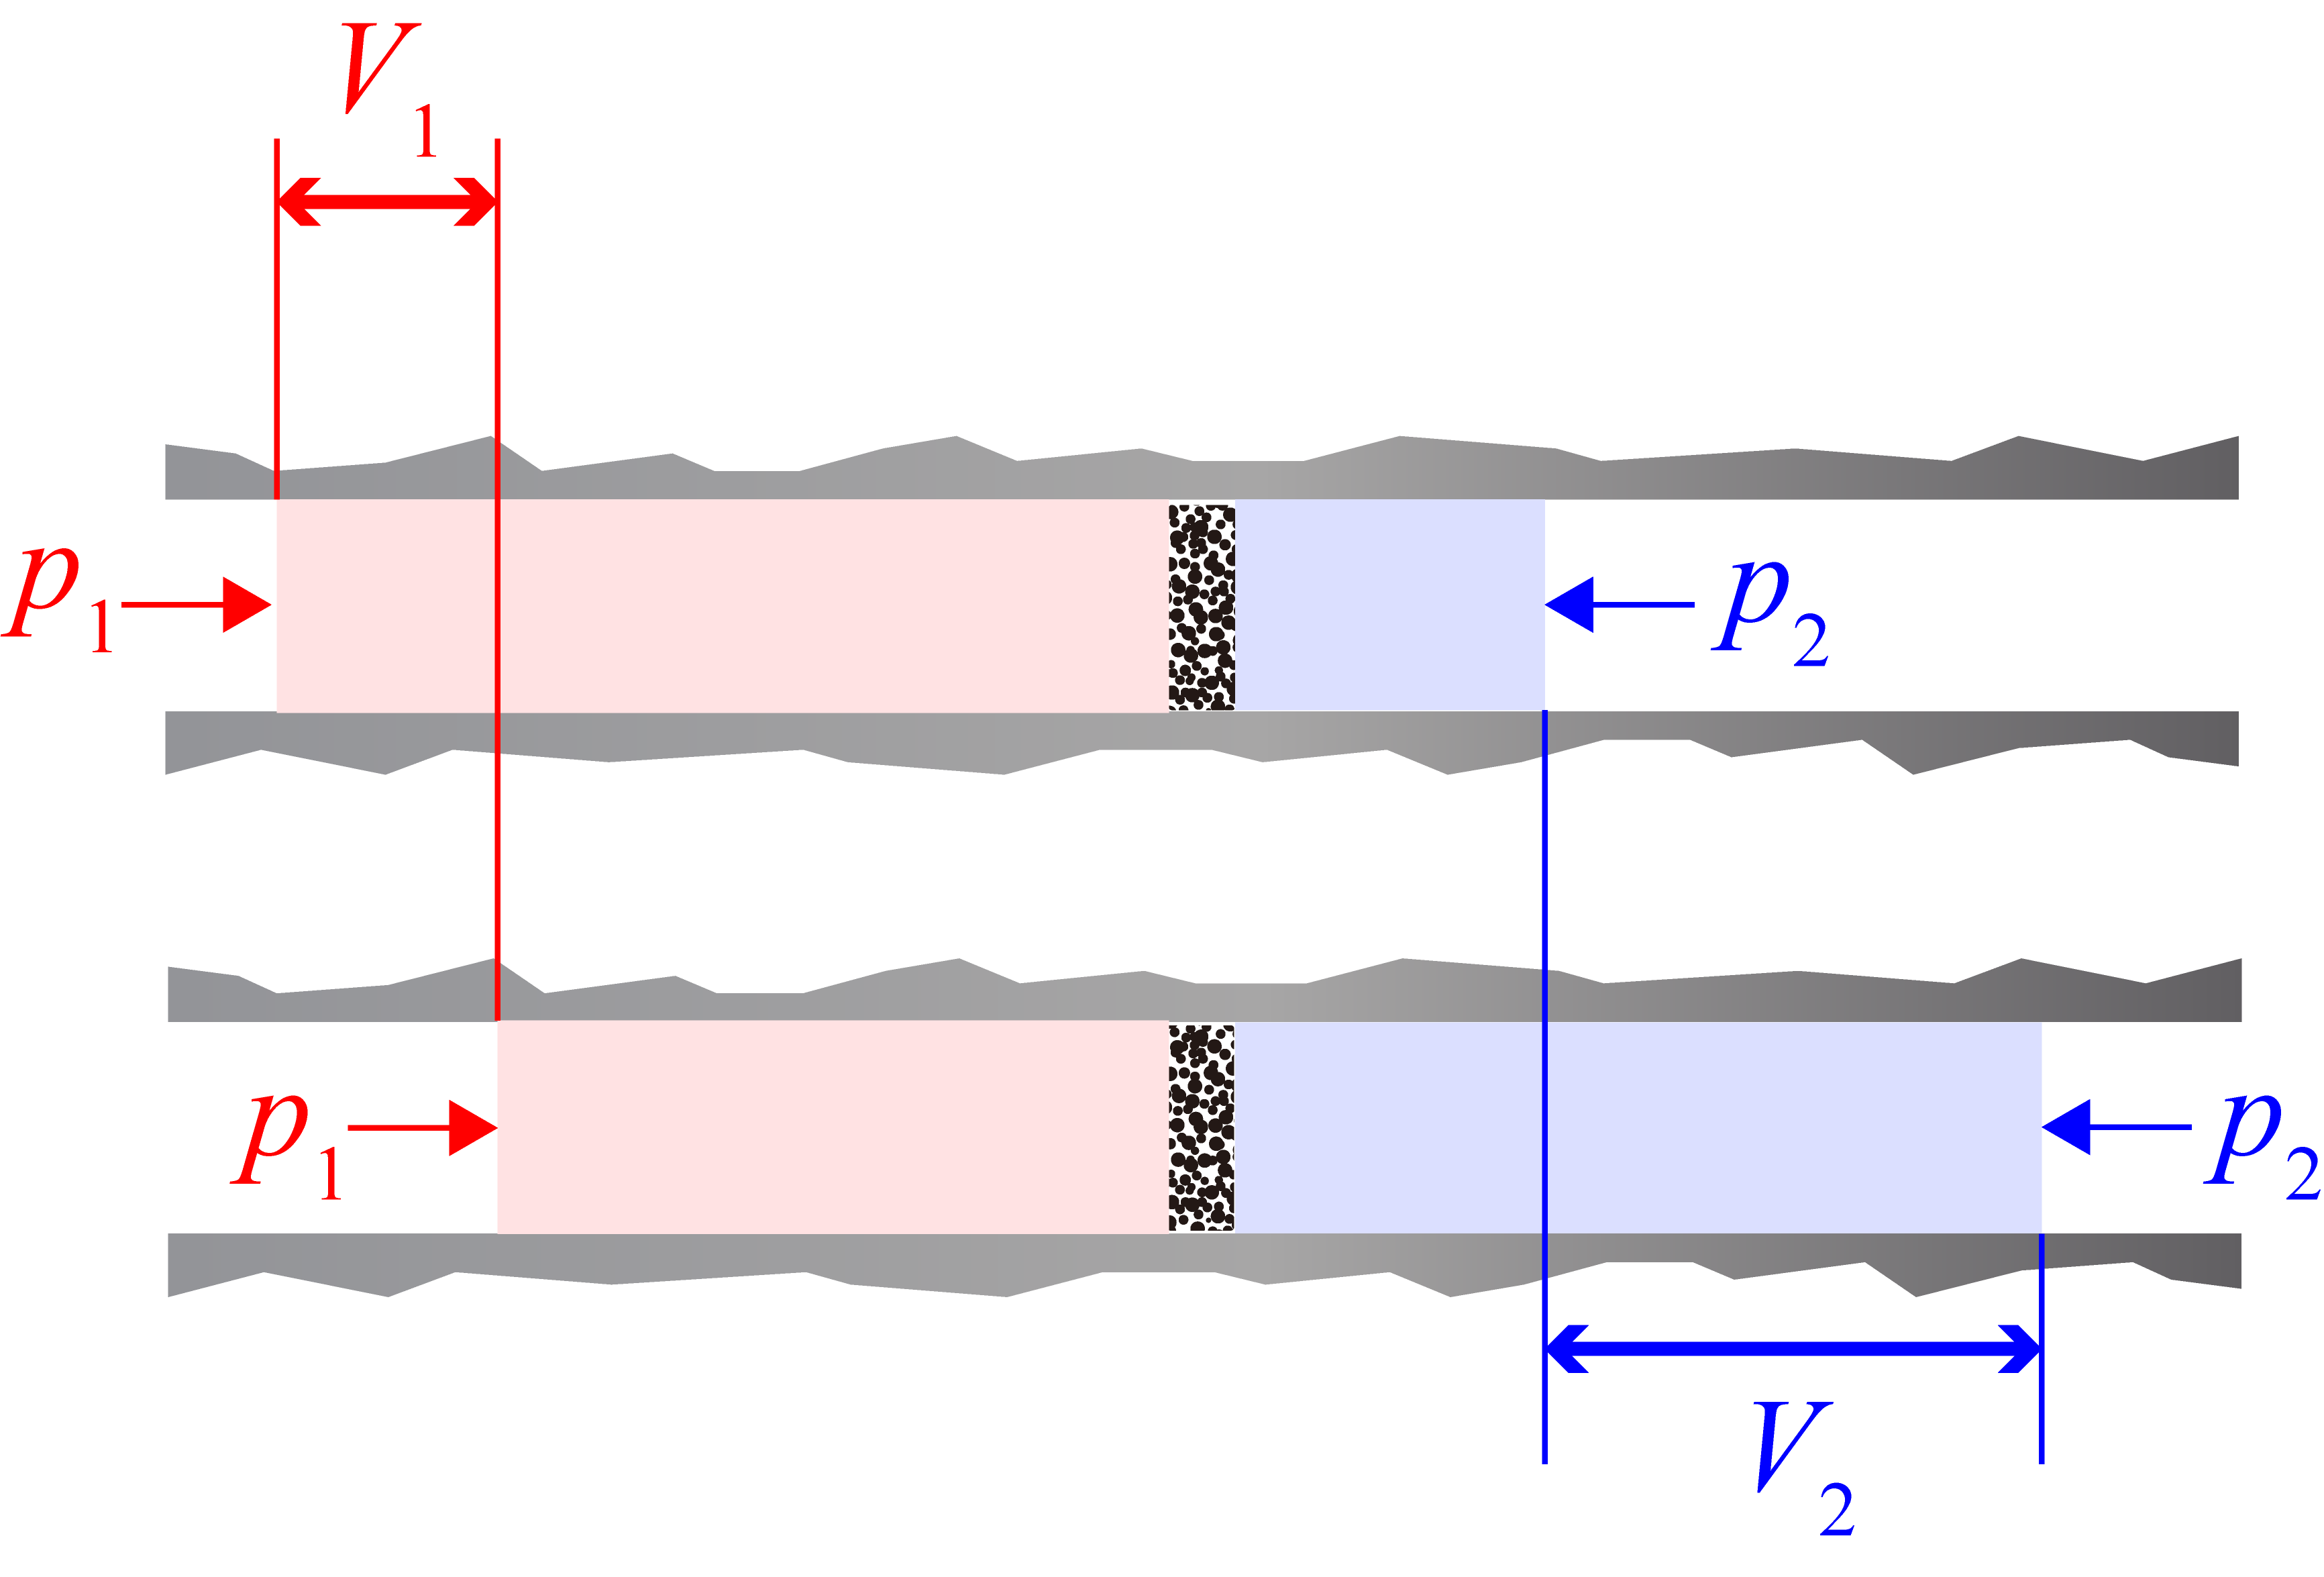
\includegraphics[width=14cm]{image/5-1-9.png}
\caption{多孔塞制节流阀}
\end{figure}

对于红+蓝的整体,\,热一定律表述为:
\[p_1V_1-p_2V_2=U_2-U_1\]

即:
\[U_1+p_1V_1=U_2+p_2V_2\quad ;\quad H_1=H_2\]

也就是说,\,节流过程前后焓不变的过程.\,若流过的气体是理想气体,\,那么
\[H=\nu C_{mV}T+pV=\nu (C_{mV}+R)T=\nu C_{mp}T\]

可见这也是一个温度不变的过程.\,但是吸热,\,做功都为零,\,它并不是一个达到平衡的准静态过程.

\npg{-2cm}

\section{开放系统的理想气体}

开放的气体系统一般有两个特点,\,一是其性质一般被描述为:\,在某处$\bs{r}$的气体性质怎样.\,而描述该气体性质的只能是各种强度量.\,如压强$p(\bs{r})$,\,温度$T(\bs{r})$等等.\,二是气体往往处于动态的物质,\,能量的交换与流动中.\,这就意味着我们分析其物理规律时必须单独取出一个\emph{气团}(parcel of air)作为研究对象.\,研究周围气体对它可能造成的微观扩散,\,黏滞,\,传热过程,\,研究周围气体对气团压力造成的体积功与加速过程.\,下面我们由简入难地分析这些问题.

\subsection{静态平衡问题\ca 重力场中的大气}
对于静态平衡的热力学体系,\,气团首先要符合的是静力学平衡条件:
\[\nabla p+\bs{f}=\bs{0}\]

其中$\bs{f}$代表体积力,\,我们考虑重力场系统,\,则为:
\[\nabla p+\rho \bs{g}=\bs{0}\]

而密度反过来又同时和压强,\,温度有关:
\[\rho=\frac{\mu p}{RT}\]

\begin{wrapfigure}[20]{o}[-10pt]{4cm}
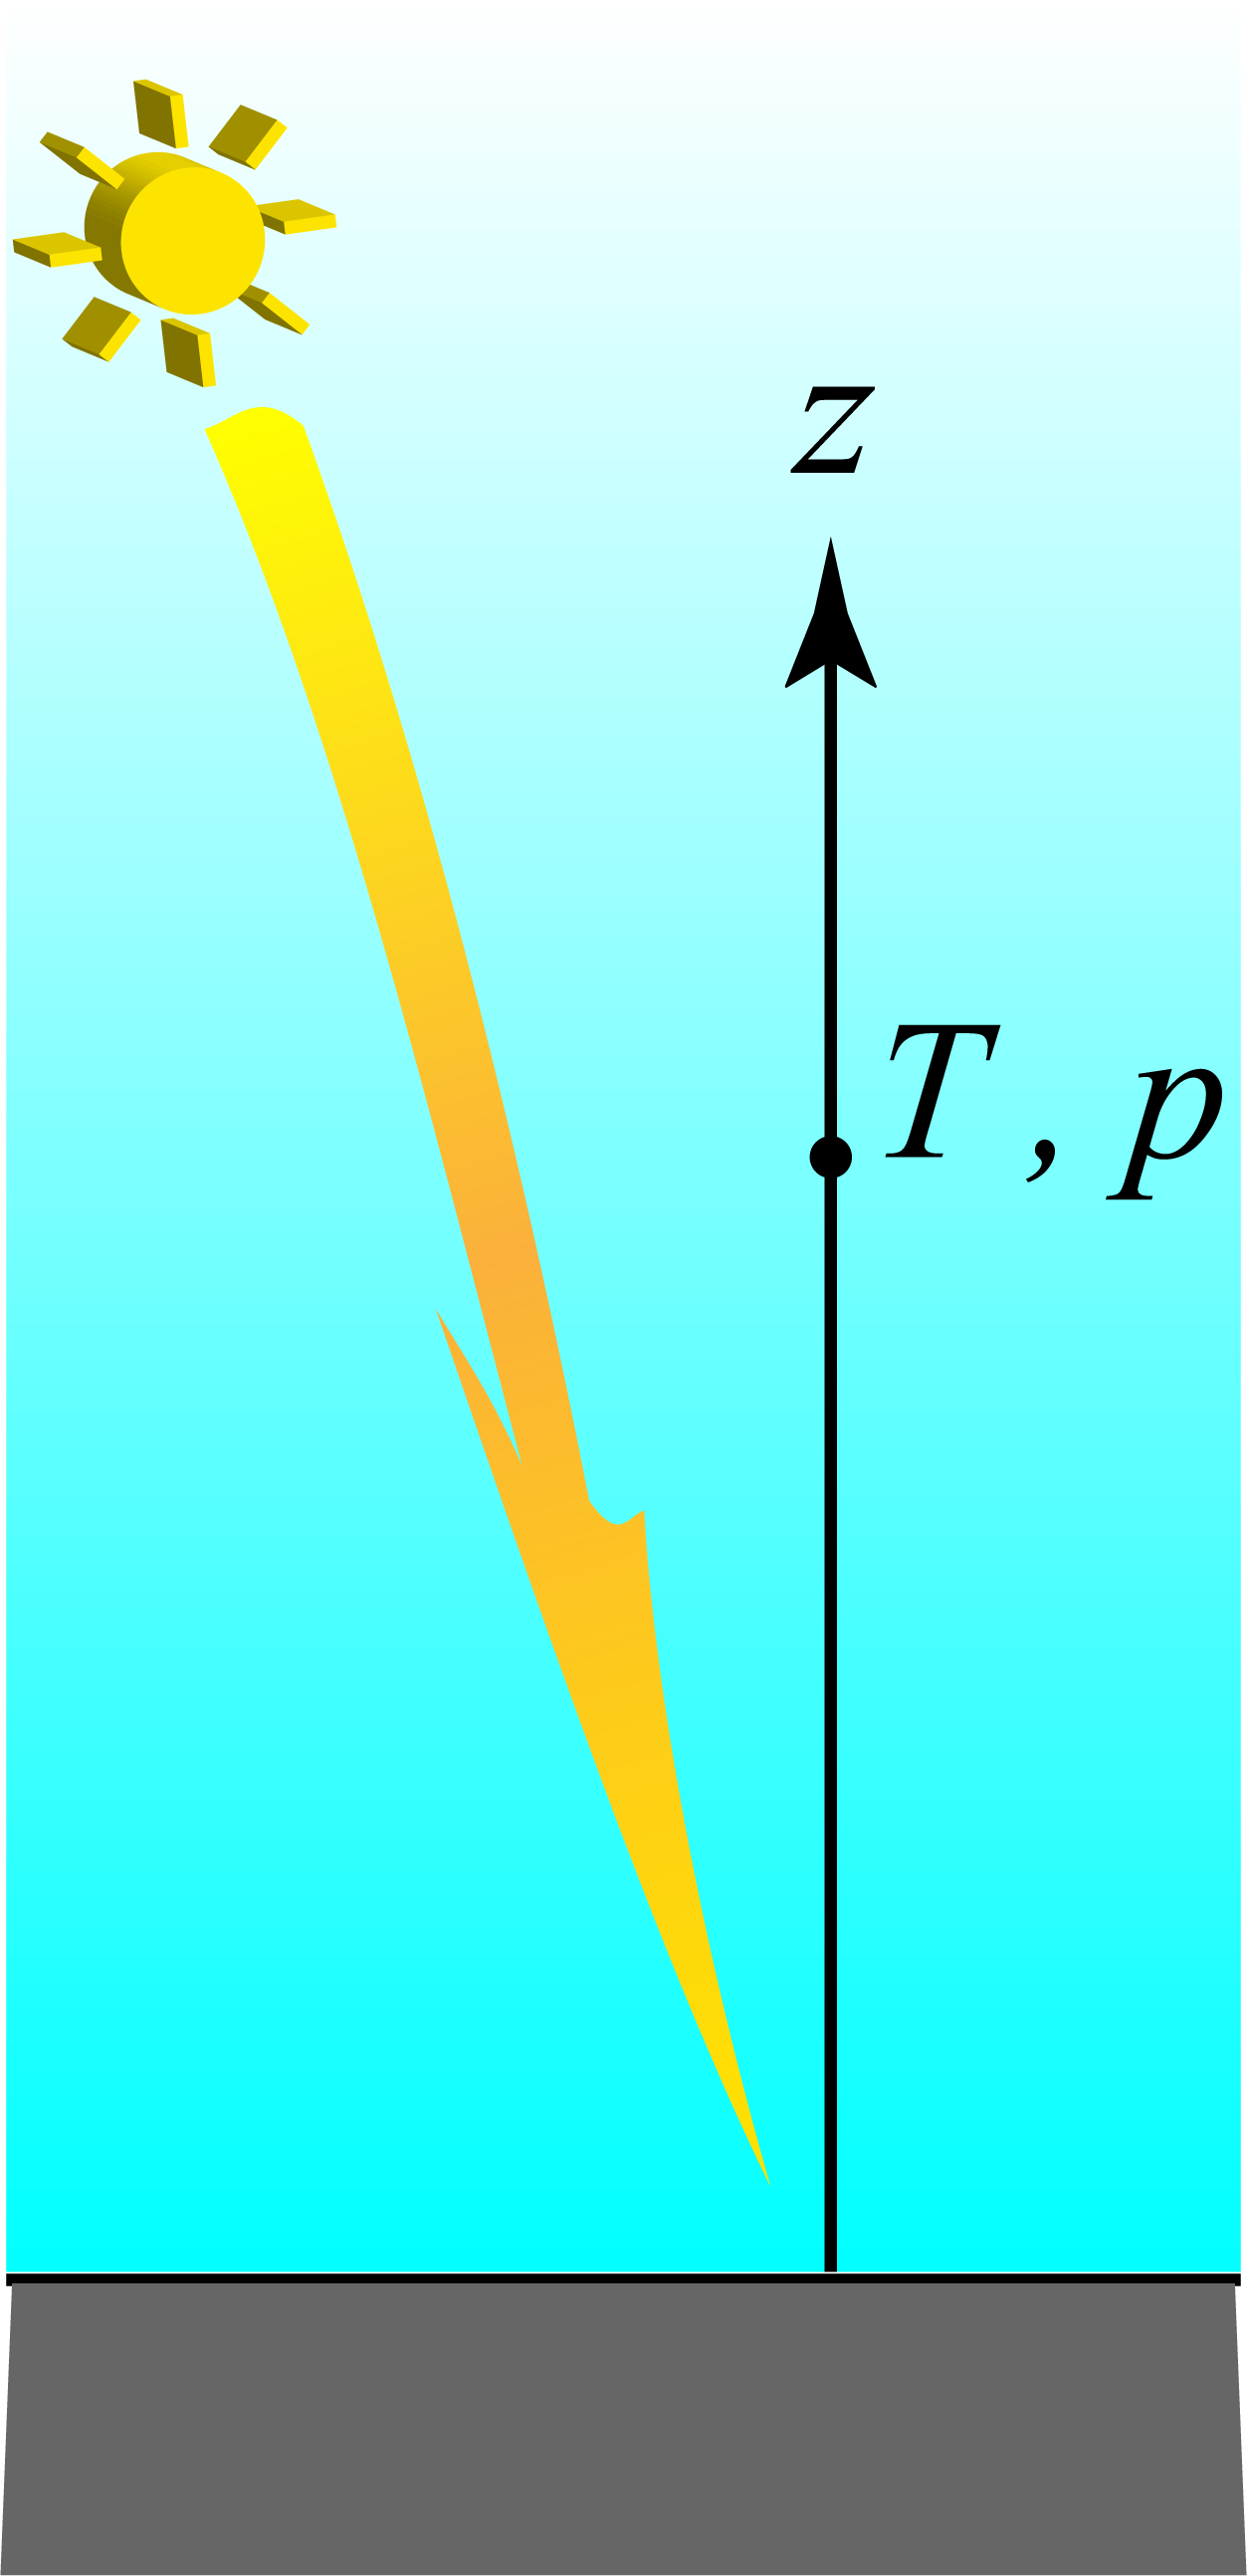
\includegraphics[width=4cm]{image/5-1-10.png}
\caption{地球大气}
\end{wrapfigure}
于是,\,压强的分布纯粹由温度分布决定,\,而温度分布则看似成为了一个纯粹的热学问题,\,而且在一定范围内粗略地研究我们可以简单地假设温度随高度均匀地变化$T(z)=T(0)-\Gamma z$.\,然而这个问题并不简单,\,大体上如果讨论限于地球表面对流层的大气,\,其基本图像可以视为由太阳照射地表,\,地表升温而加热大气导致的.\,而对于不同的气候,\,地理环境,\,时间与天气条件这个温度随高度递减的方式都十分地不相同,\,我们也还是定义\emph{环境温度递减率}(environmental lapse rate)来线性表示温度的降低:
\[\Gamma=-\frac{\ud T}{\ud z} \quad;\quad T(z)=T(0)-\Gamma z\]

了解这一点后便可计算出其压强分布:
\[p(z)=p(0)\cdot[1-\frac{\Gamma z}{T(0)}]^\frac{\mu g}{\Gamma R}=p(0)\cdot[\frac{T(z)}{T(0)}]^\frac{\mu g}{\Gamma R}\]

当环境递减率取某些不同的值时大气的性质是不同的,\,我们考虑其对流性质.\,考虑一个干的气团,\,让它在垂直方向上发生微扰,\,认为力学平衡总是很快地达到\ca 气团压强始终等于外大气压.\,但热学平衡总是来不及达到\ca 既使气团温度与外大气不相等,\,它与外界的热量交换可以忽略,\,从而可以发现,\,气团做绝热碰撞:
\[p(z)=p(0)\cdot[\frac{T'(z)}{T(0)}]^\frac{\gamma}{\gamma -1}\]

比对气团温度$T'(z)$与外大气温度$T(z)$,\,我们发现有一临界的环境温度递减率,\,我们称为\emph{干绝热递减率}(dry adiabtic lapse rate),\,它表征干燥的气团发生微扰后温度,\,密度恰好与周围大气相等的情况:
\[\Gamma_d=\frac{\gamma-1}{\gamma}\frac{\mu g}{R}=\frac{\mu g}{C_{mp}}=9.8\cdgr/\mathrm{km}\]

若$\Gamma>\Gamma_d$,\,则环境递减率过高,\,向上微扰的气团温度高于环境温度,\,所受浮力偏大,\,将偏离平衡位置,\,产生热对流,\,成云致雨.\,反之,\,$\Gamma<\Gamma_d$时浮力偏小,\,气团受到回复力而稳定在平衡位置处,\,对应着稳定无对流的大气.\,对于地球大气体系,\,有对流与无对流的情况都有时发生,\,其平均递减率就在临界绝热递减率附近.

对于临界大气为何温度随高度线性递减,\,而递减率又与定压热容有直接的关联,\,有一种较为直接的证明方法.\,其思想为虚功原理结合下面经常使用的流管分析法.\,我们让从$z=0$到$z=h$的截面积为$A$的气柱在顶部与底部的压力作用下向上发生虚位移,\,由于是临界平衡,\,故位移以后恰巧每一小块气柱$A\ud z$都与新的位置的环境大气性质全同,\,也就是与之前在这儿的那块气柱性质一样.\,整体上看,\,相当于把$z=0$处的一块质量为$\delta m$的气团位移到了$z=h$处.\,写出热力学第一定律,\,要注意其本质为能量守恒,\,这里还要包括重力势能:
\[p(0)\delta V(0)-p(h)\delta V(h)=\delta U(h)-\delta U(0)+\delta m gh\]

而由焓的定义$\delta H=\delta U +p\delta V$,\,以及理想气体的焓有公式$\delta H=\delta \nu C_{mp}T$,\,我们得出:
\[\delta \nu C_{mp}[T(0)-T(h)]=\delta \nu \mu gh\]

即:
\[T(h)=T(0)-\frac{\mu g}{C_{mp}}h\]

对于实际地球对流层大气来说,\,还需要考虑空气中水蒸气受冷造成的液化放热现象,\,其临界递减率将会取决于气体含水蒸气的多少.\,而地球下层大气还分为\emph{对流层}(troposphere)与\emph{平流层}(stratosphere),\,平流层含大量臭氧,\,太阳的紫外辐射将在传播的过程中被平流层逐渐吸收.\,所以平流层的上部具有较强的辐射和较高的平衡温度,\,而温度随高度递增,\,提供了一个稳定的大气环境,\,极难发生对流.





\subsection{能量守恒\ca 伯努利方程}
我们把流体力学里讨论的\emph{伯努利方程}(Bernoulli Equation)推广到热力学中.\,它适用条件为\emph{定常流动}(steady flow)中的同一条\emph{流线}(streamline)上.\,它也是推广的热力学第一定律,\,它代表能量的守恒.

\begin{wrapfigure}[10]{o}[-10pt]{6cm}
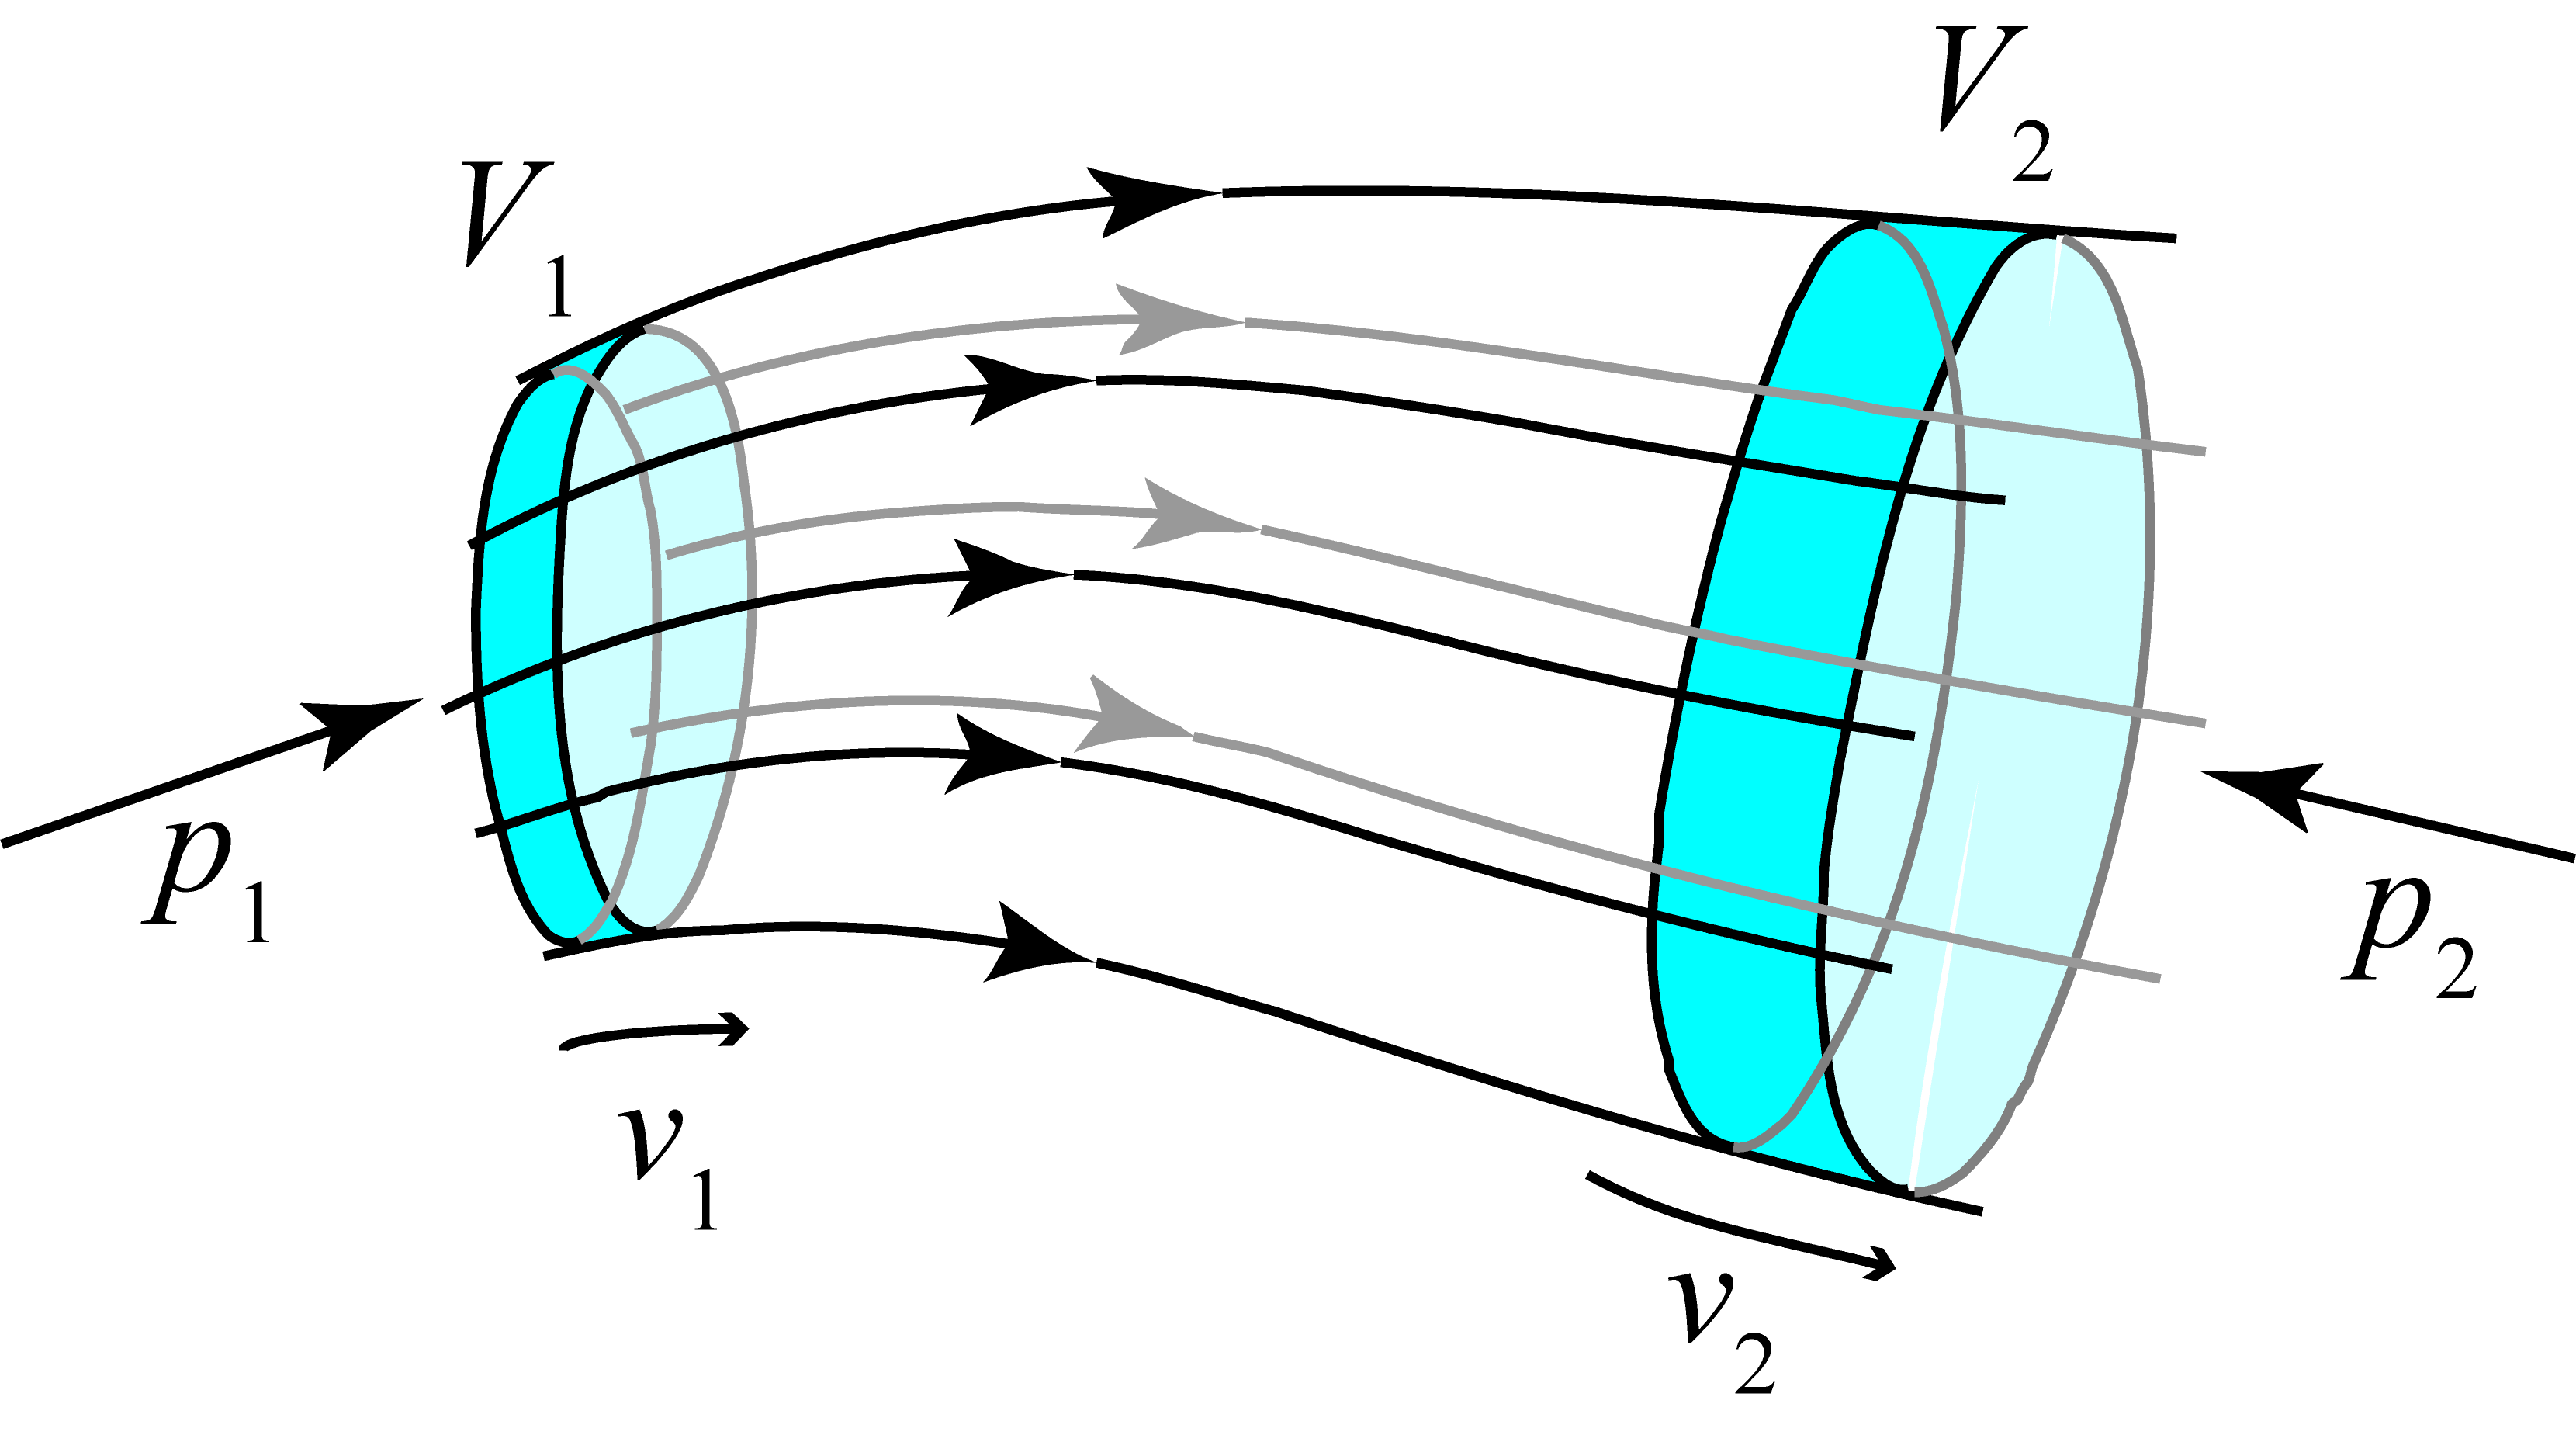
\includegraphics[width=6cm]{image/5-1-11.png}
\caption{气体沿一条流管流动}
\end{wrapfigure}
不可压缩流体的伯努利方程的图像其实很清晰,\,我们若不考虑流体势能的变化,\,那么伯努利原理实际是在说,\,两侧的压强差导致了流体的加速:
\[p_1-p_2=\frac{1}{2}\rho v_2^2-\frac{1}{2}\rho v_1^2\]

从而沿流线,\,以下量守恒:
\[p+\frac{1}{2}\rho v^2=\mathrm{const.}\]

但若考虑可以压缩的气体,\,以及考虑保守外力的做功,\,是否有以上守恒量呢?\,我们假设保守外力为质量力:\,单位质量的流体的势能为$\Phi$,\,那么对于一定时间间隔$t$下的流管发生的流动$m=Qt$,\,有以下能量守恒:
\[p_1V_1-p_2V_2=(U_2+\frac{1}{2}mv_2^2+m\Phi_2)-(U_1+\frac{1}{2}mv_1^2+m\Phi_1)\]

两边同时除以质量,\,得守恒律:
\[u+\frac{p}{\rho}+\frac{v^2}{2}+\Phi=\mathrm{const.}\]

其中$u+p/\rho=u+pv=h$即为比焓,\,而$u$为比内能,\,$v$为比体积,\,``比''表示单位质量的某物理量,\,它是一种强度量.\,从而以上量我们还可以写为:
\[h+\frac{v^2}{2}+\Phi=\mathrm{const.}\]

我们还定义所谓的\emph{阻滞焓}(stagnation enthalpy)的概念.\,它表示让运动的气体发生某种虚构的定常流动绝热地停止下来后气体应该有的焓.\,那么比阻滞焓为:
\[h'=h+\frac{v^2}{2}\]

最后这一广义的伯努利方程,\,就被我们写为一个广义的两项的能量守恒形式:
\[h'+\Phi=\mathrm{const.}\]

那么对于理想气体,\,我们还可以定义阻滞温度:
\[T'=T+\frac{\mu v^2}{2C_{mp}} \quad ; \quad h'=\frac{1}{\mu}C_{mp}T'\]

而对于普通不可压缩流体,\,我们一般不关心其热学性质,\,故焓可以扣除内能项$h=p/\rho +v^2/2$,\,而$\rho$为常数.\,这样我们又可以定义阻滞压强:
\[p'=p+\frac{1}{2}\rho v^2\quad;\quad h'=\frac{p'}{\rho}\]




\subsection{动量守恒\ca 欧拉方程}
让我们考虑管道内的理想气体流动,\,管道的截面积在不断减小的情况$A=A(x)$.\,可以想见,\,这会导致流速的增加,\,进一步导致压强的减小,\,对应方程为\emph{连续性方程}(continuity equation)与伯努利方程,\,分别对应质量与能量守恒:
\[\rho vA=\mathrm{const.}\]
\[\frac{1}{\mu}C_{mp}T+\frac{v^2}{2}=\mathrm{const.}\]

以上方程还应联系物态方程理解:
\[\rho=\frac{\mu p}{RT}\]

\begin{figure}[H]
\centering
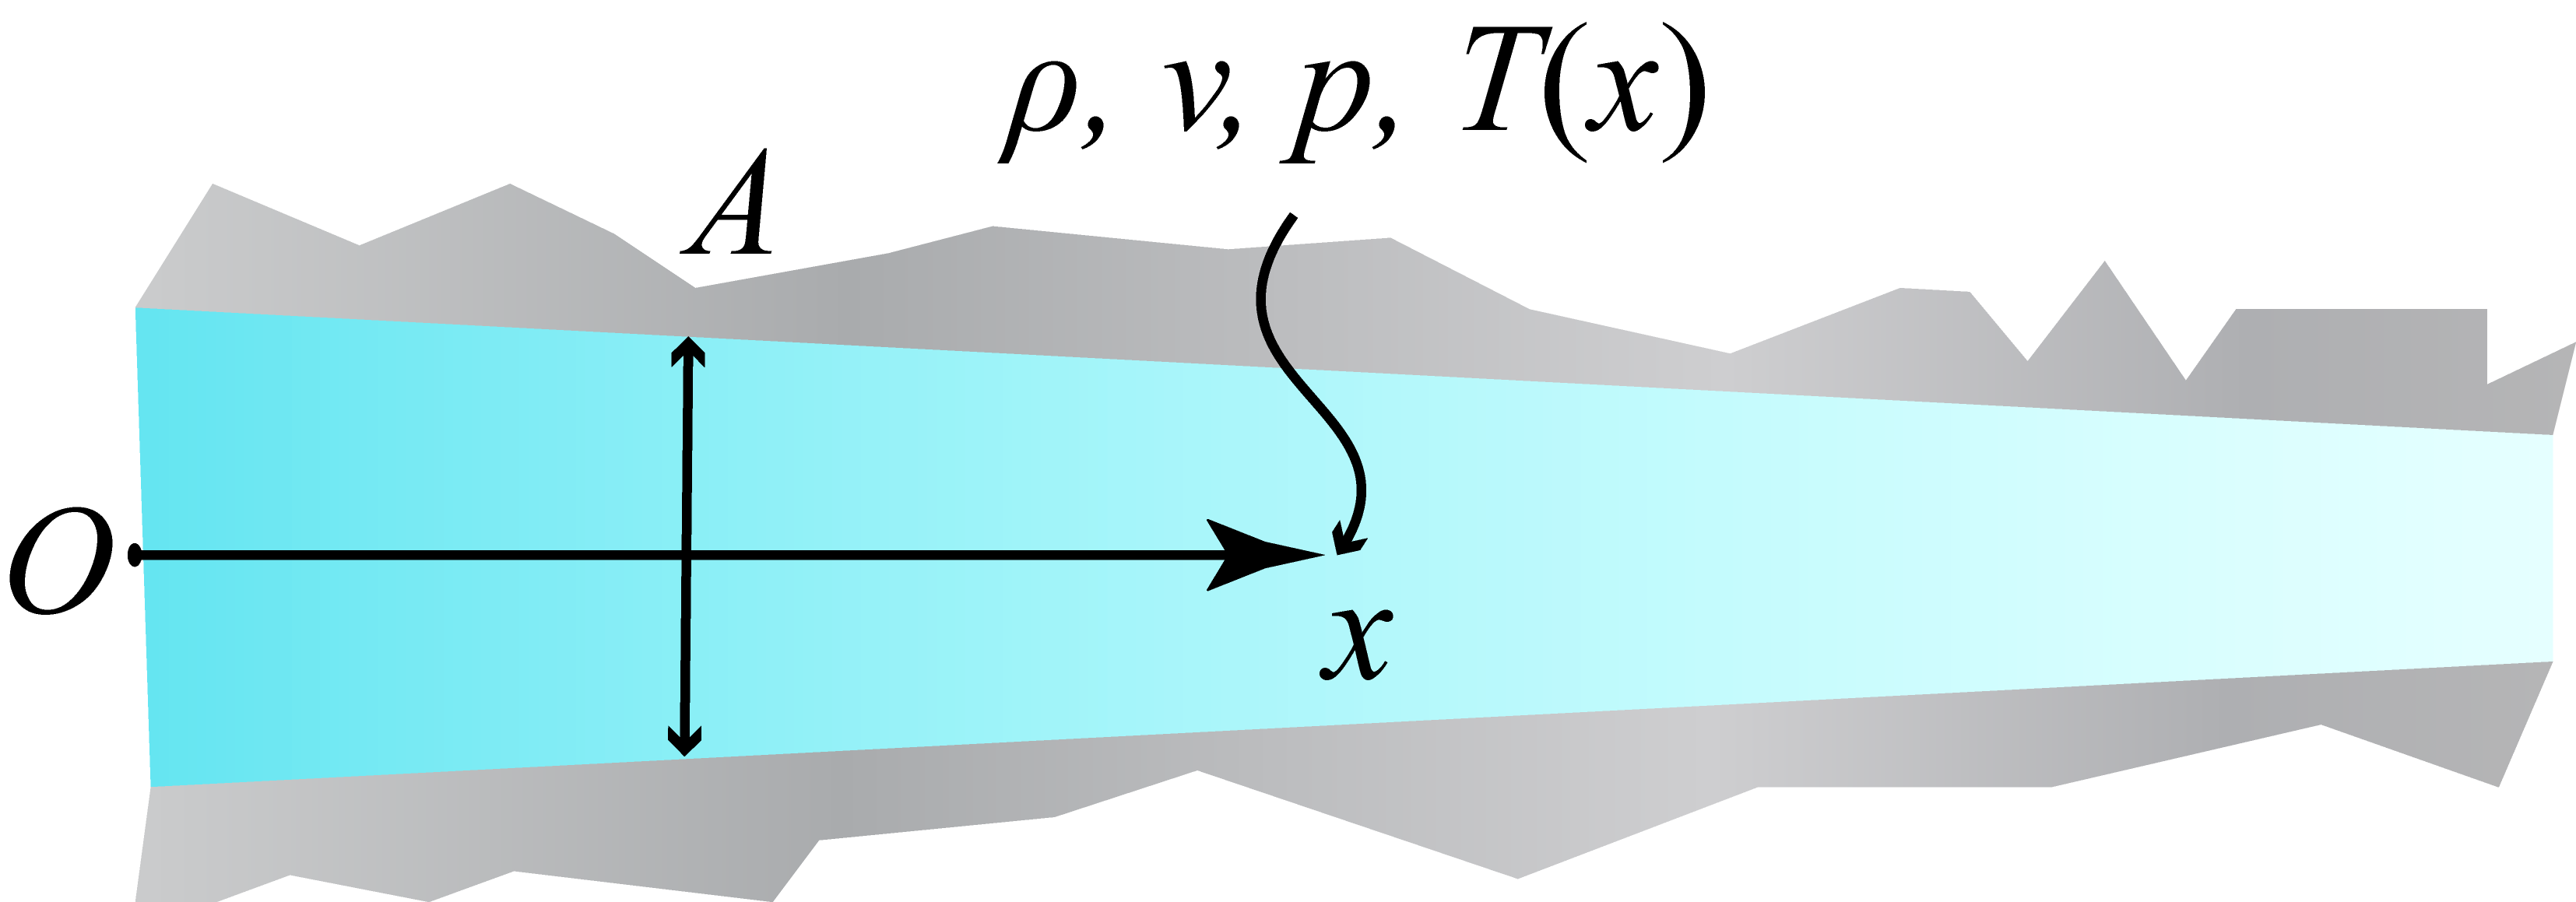
\includegraphics[width=12cm]{image/5-1-12.png}
\caption{截面积减小的管道内的气流}
\end{figure}



注意到我们把$A$的变化当做已知量以后,\,却仍设了待求解的四个物理量$v(x),\,p(x),\,T(x),\,\rho(x)$,\,但目前却只有三个方程.\,那么我们漏了怎样一个方程呢?\,这个方程就是流体的\emph{欧拉方程}(Euler equation),\,它是一个纯粹的动力学方程,\,不包含任何热效应.\,一般写作:
\[\frac{\mathrm{D} \bs{v}}{\mathrm{D} t}=-\frac{\nabla p}{\rho}-\nabla \Phi\]

其中$\mathrm{D}$代表\emph{随体导数}(material derivative):
\[\frac{\mathrm{D}}{\mathrm{D} t}=\frac{\ud}{\ud t}+\bs{v}\cdot \nabla\]

上式代表了压强梯度力与保守外力对流体的加速效应,\,在上述情形中没有外力所以等式右边只有一项.\,实际上,\,它代表了整个体系动量守恒.\,而对于上述情形,\,气体做定常流动,\,上式写为:
\[v\frac{\ud v}{\ud x}=-\frac{1}{\rho}\frac{\ud p}{\ud x}\]

这一个式子也可以由上一节的类似方法\ca 取一定长度的气团来导出.\,但切不可忽略管壁对气体在过程中作用的冲量:
\[p_1A_1\bs{e}_x \cdot t-p_2A_2\bs{e}_x \cdot t+\int -p\ud \bs{A} \cdot t=m\bs{v}_2-m\bs{v}_1\]

左边恰巧是在整个表面的压强的面积分,\,可以由高斯定理化为体积内的体积分:
\[\int_{x_1}^{x_2}-\frac{\ud p}{\ud x}\cdot A\ud x=Q(v_2-v_1)\]

又考虑到以上积分式无法直接积出结果,\,故对积分上限求导,\,再考虑到$Q=\rho vA$,\,化简后即得欧拉方程:
\[\frac{\ud p}{\ud x}=-\rho v\frac{\ud v}{\ud x}\]

对于管道截面积相对于长度变化缓慢的情况\footnote{即,\,在所关心的范围内截面积的相对变化很小:\[\frac{\Delta A}{A}\ll 1\]},\,联立以上四个方程,\,解得:
\[\frac{\ud v}{v}=-\frac{\ud A}{A}(1-\frac{\mu v^2}{\gamma RT})^{-1}\]
\[\ud p=\rho v^2\cdot\frac{\ud A}{A}(1-\frac{\mu v^2}{\gamma RT})^{-1}\]
\[\ud T=\frac{\mu v^2}{C_{mp}}\cdot\frac{\ud A}{A}(1-\frac{\mu v^2}{\gamma RT})^{-1}\]

可见,\,随着截面积$A$的减小,\,流速加快,\,压强和温度都要减小,\,利用这个效应可以制作纯粹依靠风力制冷的``土空调''.\,注意到以上结论还依赖于一个条件:
\[\frac{\mu v^2}{\gamma RT}<1\]

这意味着分子代表的气团集体运动能量要远小于分母代表的微观热运动能量,\,这在一般情况下是很容易满足的,\,因为$v\sim 10 \mathrm{m/s}$而热运动平均速率$\bar{v}\simeq 500 \mathrm{m/s}$,\,若对于高速运动的气体,\,其发生的过程中气团速度的改变与热运动平均速度可以比拟,\,实际上把气团处理为平衡的理想气体也是不妥当的.